% !TEX root = ../main.tex
% Chapter 1
\flushleft
\chapter{Cut Glue and Cut Algorithm}\label{ch:cgc} 





%%%%%%%%%%%%%%%%%%%%%%%%%%%%%%%%%%%%%%%%%%%%%%%%%%%%%%%%%%%%%%%
%                                                             %              
%      ABSTRACT                                               %  
%                                                             %                  
%%%%%%%%%%%%%%%%%%%%%%%%%%%%%%%%%%%%%%%%%%%%%%%%%%%%%%%%%%%%%%%
Recently, unsupervised image segmentation has become increasingly popular.
Starting from a superpixel segmentation, an edge-weighted region adjacency graph is constructed. 
Amongst all segmentations of the graph, the one which best conforms to the given image
evidence, as measured by the sum of cut edge weights, is chosen.

Since this problem is NP-hard, we propose  a new approximate solver based on the move-making paradigm:
first, the graph is recursively partitioned into small regions (cut phase).
%
Then, for any two adjacent 
regions, we consider alternative cuts of these two regions
defining possible moves (glue \& cut phase).
%
For planar problems, the optimal move can be found, whereas
for non-planar problems, efficient approximations exist. 

We evaluate our algorithm on published and
new benchmark datasets.
%
The proposed algorithm finds segmentations that,
as measured by a loss function, are as close to
the ground-truth as the global optimum found by exact solvers.
%
It does so significantly faster then existing approximate methods,
which is important for large-scale problems.








%%%%%%%%%%%%%%%%%%%%%%%%%%%%%%%%%%%%%%%%%%%%%%%%%%%%%%%%%%%%%%%
%                                                             %              
%      Introduction                                           %  
%                                                             %                  
%%%%%%%%%%%%%%%%%%%%%%%%%%%%%%%%%%%%%%%%%%%%%%%%%%%%%%%%%%%%%%%
\section{Introduction}


Segmentation is an important problem in computer vision as a first step
towards understanding an image. Many algorithms start with an over-segmentation
into superpixels, which are then clustered into ``perceptually meaningful''
regions.
Usually, the number of these regions is not known beforehand.

Recently, the multicut formulation~\cite{chopra_1993_mp}
(sometimes called \emph{correlation clustering}, \cite{bansal_2004_ml})
has become increasingly popular for unsupervised
image segmentation.
Given an edge-weighted region adjacency graph,
the problem is to find the segmentation which
minimizes the cost of the cut edges.
Such an approach has been shown to yield
state-of-the-art results on the Berkeley Segmentation Database
%TODO: - alush_2013_simbad apply it on BSD500, is is state-of-the-art?
%      - gPb-owt is not really learned? Do we need to say this????
\cite{andres_2011_iccv,yarkony_2012_eccv,alush_2013_simbad}.

Unfortunately, solving the multicut problem is in general NP-hard.
Any exact solver will therefore be plagued by scalability issues.
However, segmentation of images with ever finer superpixel
partitionings and of large volume images in computational neuroscience 
\cite{kroeger_2012_eccv}
demand solutions to large scale multicut problems.
%
In this regime of large-scale problems, existing solvers either
fail to find any solution after a reasonable time,
rely on suitable edge weights (such that the problem decomposes naturally
into independent subproblems) 
or yield an approximate solution possibly far away from the optimum.

\vspace{0.1cm}
\noindent
\textbf{Contribution.}
In this work we consider 
\begin{inparaenum}[(i)]
\item
a new perspective on solving the multicut problem by
\emph{local} move making methods together with
%
\item
a new approximate multicut solver called
\emph{Cut, Glue \& Cut (CGC)}. Furthermore,
%
\item our method avoids re-solving the same moves
by tracking their ``dirtyness'', which decreases the runtime. 
%
\item
An extensive evaluation on existing and new benchmark datasets shows
that CGC provides results close to optimality
and equal application performance significantly faster than all its
competitors, both exact
and approximative methods, and gives new insights concerning the applicability
of competing methods.
%
\item
Our C++ implementation of CGC will be made available with release of this paper.
\end{inparaenum}

\vspace{0.1cm}
\noindent
\textbf{Organization.}
In Sec.~\ref{sec:problem_formulation} we review two common formulations
of the multicut problem. After discussing related work in
\cref{sec:gcg_related_work} and 
the max-cut problem in \cref{sec:max_cut}.
Based on a general formulation of local partition moves on segmentations in
\cref{sec:cut_moves},
we describe our new Cut, Glue \& Cut algorithm
in \cref{sec:cut_glue_cut_algorithm}. Extensive experiments
on benchmark datasets are presented in \cref{sec:experiments}.
Finally, we discuss our findings.




%%%%%%%%%%%%%%%%%%%%%%%%%%%%%%%%%%%%%%%%%%%%%%%%%%%%%%%%%%%%%%%
%                                                             %              
%      PROBLEM FORMULATION                                    %  
%                                                             %                  
%%%%%%%%%%%%%%%%%%%%%%%%%%%%%%%%%%%%%%%%%%%%%%%%%%%%%%%%%%%%%%%
\section{Problem Formulation\label{sec:problem_formulation}}
Let $G=(V,E, \w)$ be a weighted region adjacency graph of
nodes $V$, representing superpixels,
and edges $E$.
%
The function $\w : E \rightarrow \mathbb{R}$ assigns a weight to each edge.
A positive weight expresses the desire that two adjacent nodes should
be merged, whereas a negative weight indicates
that these nodes should be separated into two different regions.

A \emph{subgraph} $G_A = \{A, E_A, \w\}$ consists
of nodes $A \subseteq V$ and edges $E_A = E\cap (A\times A)$.
%
In the following, we will call a connected component
of nodes $V$ a \emph{region} $R \subseteq V$.
%
Each node $i$ is assigned a 
label $\Labels_{i} \in \{0, \dots, | V |-1\}$. Using the indicator 
function
$\delta(\cdot)$, the
\emph{multicut problem} can be written as a node labeling problem
\cite{bagon_2011_arxiv}:
%
\begin{align}
\argmin_{\Labels}
    \left\{
    \sum_{ e=(i,j) \in E}
        \w(e)
        \cdot \delta( \Labels_i \neq \Labels_j )
    \right\},
    \label{eq:multicut_primal}
\end{align}
%
where $\delta(a) = 1$ if $a$ is true and $0$ else.
%
While \eqref{eq:multicut_primal} looks like a common Potts energy without
unary terms, there are some crucial differences:

\noindent
\emph{First}, any weight $\w(e\!\in\!E)$ can be positive or negative.

\noindent
%TODO: any unary data terms? or: strong unary data terms
\emph{Second}, the lack of any unary data terms renders the problem much harder
and introduces ambiguity.

\noindent
\emph{Third}, the label space is large.
In general we have to set
$|\Labels| = |V|$ to allow for the solution
where every supervoxel becomes its own region
without having to solve the graph coloring problem implicitly.
For planar graphs, it would be sufficient that $\Labels_i \in \{0,...,3\}$
because any planar-graph is 4-colorable \cite{appel_1977_4color}.
%Ulli: 5-coloring is linear time for planar graphs
%
%Unfortunately, as the 4-coloring is itself NP-hard, this does not appear
%to make the multicut problem easier to solve.


An alternative formulation of problem \eqref{eq:multicut_primal}
is in terms of binary edge indicator variables
$\y \in \{0,1\}^{| E |}$:
\begin{align}
\argmin_{\y}
\underbrace{%
    \left\{
        \sum_{e=(i,j) \in E} \w \left(e\right) \cdot \y_{e}
    \right\}%
}_{%
    \CUT_G(\y)%
}%
\;\;\text{s.t.}\;\;\y \in \MC_G.
\label{eq:multicut_dual}
\end{align}
%
A segmentation $\y$ has an associated \emph{energy}
which is denoted by $\CUT_G(\y)$.
%
$\text{MC}_G$ is the set of all multicut
constraints \cite{chopra_1993_mp} for graph $G$ forming
the so called \emph{multicut polytope}.
These constraints ensure that labeling $\y$ is
\emph{consistent}:
%TODO: Notation: ij <-> edge e
if $\y_{ij}=1$ then nodes $i$ and $j$ should be in
separate regions even after connected component labeling. Intuitively,
dangling line segments are forbidden in two dimensional images,
and punctured walls or faces are ruled out in three dimensional images.

While any segmentation $\bigcup_{i} R_i \equiv V$ is represented by exactly one
edge labeling $\y\in\MC_G$, many labelings $\Labels$ represent the same segmentation.
Therefore, a multicut representation \eqref{eq:multicut_dual} is preferrable
to avoid large multiplicities of local optima.
%
However, an efficient handling of the multicut polytope is
essential.





%%%%%%%%%%%%%%%%%%%%%%%%%%%%%%%%%%%%%%%%%%%%%%%%%%%%%%%%%%%%%%%
%                                                             %
%      RELATED WORK                                           %
%                                                             %
%%%%%%%%%%%%%%%%%%%%%%%%%%%%%%%%%%%%%%%%%%%%%%%%%%%%%%%%%%%%%%%

\section{Related Work\label{sec:gcg_related_work}}
Applying state-of-the-art solvers for the labeling
problem~\eqref{eq:multicut_primal} is challenging since any permutation of
the labelings transforms an optimal solution into another optimal solution,
see \cite{kappes_2013_arxiv} for more details and a recent review.
%TK TODO: What about bagon_2011_arxiv?
%         Shouldn't we a bit more kind towards that method?

%which are handled by a cutting plane procedure,
%\cf~\cite{kappes_2013_arxiv,kappes_2011_emmcvpr, andres_2011_iccv, kim_2011_nips}.
% + exponential number

In general,
$\y \in \MC_G$ can be enforced by an exponential number of
constraints \cite{chopra_1993_mp}, but in practice
-- for a given objective function --
a small subset of those are sufficient.
Therefore, a major branch of research has focused 
on cutting plane approaches,
either by solving a relaxation of \eqref{eq:multicut_dual}
by a sequence of linear programs 
\cite{kim_2011_nips,kim_2012_ip,kappes_2013_arxiv,finley_2005_ml} 
or
by solving problem \eqref{eq:multicut_dual} exactly by a sequence
of integer linear programs
\cite{kappes_2011_emmcvpr,andres_2011_iccv,kroeger_2012_eccv,kappes_2013_arxiv,alush_2012_pami,alush_2013_simbad}.
%These sequences are
%interleaved with separation procedures 
%that provide additional, violated constraints.

For the latter, one can avoid the cutting plane procedure by lifting to the
fully connected graph at the expense of problem size \cite{alush_2012_pami}.
For many image segmentation problems, however, the size of the complete graph is
prohibitively large.

Alush and Goldberger \cite{alush_2012_pami,alush_2013_simbad} suggest to use
partial optimality in order to decompose the
problem into its positively connected components,
defined as the connected components of the graph $G'=(V,E')$ with
$E'=\{e\in E | \w_e > 0 \}$.
These problems are then separately solved to global optimality.
While this recovers the true solution, it depends on
the weights $\w$ whether 
a significant reduction of the problem is possible.

Yarkony et al.~\cite{yarkony_2012_eccv} suggest a method,
called PlanarCC,
which solves a relaxed linear program by
iteratively solving weighted two-coloring problems.
Because these sub-problems require planarity to be tractable,
PlanarCC is restricted to problems with planar structure.

%TODO: leave this commented?
%\iffalse
When the formulation as a complete graph
with $| E | \sim O(| V|^2)$
is feasible, \eqref{eq:multicut_dual} can be solved by an integer linear program with
$| V|^3$ triangle constraints \cite{chopra_1993_mp,alush_2012_pami,finley_2005_ml}.
\todo{check chopra ref}.
For image segmentation problems, however, the size of the complete graph is
prohibitively large.
%\fi

%
%TK TODO: check finley_2005_ml
%TODO: leave this out?
%Kroeger et al. describe a heuristic of decomposition into overlapping blocks
%\cite{kroeger_2013_miccai}. 

Another branch of research has focused on specialized move-making methods
\cite{kerninghan_1970_bell,zhao_2005_mp,bagon_2011_arxiv}
that take the degeneracy of the solution,
due to label permutations in \eqref{eq:multicut_primal}, into account.
%
Move-making algorithms maintain a valid solution (segmentation defined 
via $\Labels$ or, equivalently, $\y \in \MC$) throughout the
optimization procedure. In each step, a set of possible moves transforming
the current segmentation is considered,
and the move which realizes the maximal
energy decrease is chosen. Therefore, the energy decreases monotonically
until a (local) optimum is found.
%
The Kerninghan-Lin method~\cite{kerninghan_1970_bell},
used in circuit-layout design, applies a sequence of 
greedy local moves to neighboring regions.
Bagon~\cite{bagon_2011_arxiv} recently proposed an 
extension to the
$\alpha$-expansion move-making algorithm
for solving multicut problems, which handles the large label space
and label ambiguity in \eqref{eq:multicut_primal} by using dynamic label
sets and additional label fixing, respectively.







%%%%%%%%%%%%%%%%%%%%%%%%%%%%%%%%%%%%%%%%%%%%%%%%%%%%%%%%%%%%%%%
%                                                             %
%      MAX CUT                                                %
%                                                             %
%%%%%%%%%%%%%%%%%%%%%%%%%%%%%%%%%%%%%%%%%%%%%%%%%%%%%%%%%%%%%%%
\section{Max-Cut\label{sec:max_cut}}
A basic subproblem which has to be solved in
the Kerninghan-Lin method \cite{kerninghan_1970_bell},
Expand-and-Explore \cite{bagon_2011_arxiv},
PlanarCC \cite{yarkony_2012_eccv} and also our method is the
max-cut problem \cite{deza1997geometry} (also known as weighted 2-coloring).

The max-cut problem\footnote{%
For reasons of consistency, we consider wlog. minimization instead of maximization.
}
is the specialization of \eqref{eq:multicut_primal}
for the case of binary node labels $\Labels_i = \{0,1\}$, given by
\begin{align}
\argmin_{\vec{L \in \{0,1\}^{|E|}}}
         \left\{
            \sum_{e=(i,j)\in E} \w(e)
                \cdot \delta( \Labels_i \neq \Labels_j )
         \right\}
         \label{eq:max_cut}.
%\intertext{or alternatively with $S_0 = \{v\in V | \Labels_v = 0\}$:}
%\argmin_{S_0 \subseteq V} \underbrace{%
%    \sum_{e \in E \cap (S_0\times V\setminus S_0)} \w_e}_{:=\CUT_G(S_0)}
%\label{eq:cut}
\end{align}

This should not be confused with the min-cut problem, which refers to
sub-modular ``graphcut problems'' with non-negative edge weights
$\w$, for which a max-flow problem can be formulated
\cite{kolmogorov_2004_pami}.
%
Intuitively, restricting the label space to two labels (0 and 1) simplifies the
problem.
%
For planar graphs, \eqref{eq:max_cut} can be solved by the
Blossom algorithm \cite{schraudolph_2009_nips} in polynomial time.
In general this problem is still NP-hard.
%
In response, Kerninghan and Lin have suggested a greedy method
for \eqref{eq:max_cut} used in the
KL algorithm \cite{kerninghan_1970_bell}. Recently,
Bagon~\cite{bagon_2011_arxiv} suggested to use
\mbox{QPBO-I}~\cite{rother_2007_cvpr} for \eqref{eq:max_cut}.
While this LP relaxation 
often gives to non-integral solutions for many nodes, the improving
extension (-I)~\cite{rother_2007_cvpr} iteratively fixes such nodes and
therefore also deals with the ambiguity of the problem.

In our experiments, we found that using \mbox{QPBO-I} performs 
better than the greedy method used in the KL algorithm,
but slightly worse than optimal solvers (Sec.~\ref{sec:experiments}).





%%%%%%%%%%%%%%%%%%%%%%%%%%%%%%%%%%%%%%%%%%%%%%%%%%%%%%%%%%%%%%%
%                                                             %
%     PARTION MOVE                                            %
%                                                             %
%%%%%%%%%%%%%%%%%%%%%%%%%%%%%%%%%%%%%%%%%%%%%%%%%%%%%%%%%%%%%%%
\section{Partition Moves\label{sec:cut_moves}}
\noindent
In this section we define a class of moves which can be used to iteratively
improve segmentations. The Partition Move Theorem shows that under some
technical conditions, the improvement of the local sub-problem 
leads to monotonous improvement of the global energy.

\vspace*{0.3cm}
\noindent\textbf{Theorem: \emph{Partition Moves.}}
%
Let $\y^t \in \text{MC}_G$ represent the segmentation of $G$ at step $t$.
Local partition moves are defined over a subset $S \subset V$ for which all
edges crossing its borders have to be labeled one:
$\forall\;e\in E\cap (S\times(V\setminus S)): \y_e^t = 1$.\\
%
Let $G_S$ be the respective subgraph of $G$ and
$\hat{\y} \in \text{MC}_{G_S}$ represent a given valid segmentation of $S$. 
For the combined segmentation
%
\begin{align}
{
\y^{t+1} := \begin{cases}
                  \hat{\y}_e \quad e\in E_S  \\
                  \y_e^t \quad \text{else} 
            \end{cases}%
            \label{eq:y_t_plus_one}
}%                
\end{align}
the following holds:\\
\begin{inparaenum}[(i)]
\item
{
$\y^{t+1} \in \text{MC}_G$.\\
}
\item
{
$\CUT_{G_S}(\hat{\y}_{E_S}) \leq \CUT_{G_S}({\y}_{E_S}^t) \Rightarrow
\CUT_{G}({\y}^{t+1}) \leq \CUT_{G}({\y}^t)$.}
\end{inparaenum}

\vspace*{0.2cm}
\noindent\textbf{Proof.}
(i)
Let us extend the local segmentation $\hat{\y}$ to $G$ with
\begin{align*}
{
\hat{\y}_G := \begin{cases}
                  \hat{\y}_e \quad &\forall e\in E_S\\
                  1          \quad &\forall e\in E \cap S\times (V\setminus S)\\
                  0          \quad &\forall e\in E \cap (V\setminus S)\times(V\setminus S)
            \end{cases}%
}%                
\end{align*}
%
Since (a) 
$\hat{\y}_G \in \text{MC}_G$,
(b)
$\y^{t+1} = \text{OR}(\hat{\y}_G, \y^t)$,
and (c) the 
set of multicuts is closed under the OR operation, (i) holds.\\
%
(ii)
For
$\CUT_{G_S}(\hat{\y}_{E_S}) \leq \CUT_{G_S}({\y}_{E_S}^t)$,
the energy after the move can be written as:



\begin{align*}
%\sum_{e\in E}              \w_e \y_e^1
\CUT_G(\y^{t+1})
&=
\sum_{e\in E_S}            \w(e) \y_e^{t+1} +
\sum_{e\in E\setminus E_S} \w(e) \y_e^{t+1}
\\
&\leq
%
\sum_{e\in E_S}            \w(e) \y_e^t +
\sum_{e\in E\setminus E_S} \w(e) \y_e^{t+1}\\
%
&=
%
\sum_{e\in E_S}            \w(e) \y_e^t +
\sum_{e\in E\setminus E_S} \w(e) \y_e^t 
%
=
%
\CUT_G(\y^t).\\
&\hspace*{0.75\columnwidth}
\end{align*}



To obtain an alternative segmentation $\hat{\y}$ on $G_S$, one can either
\begin{inparaenum}[(a)]
\item solve the multicut problem over $G_S$ (which is smaller than $G$)
or
\item restrict the subset of possible segmentations,
      e.g. to all two-colorable segmentations of $G_S$%
\end{inparaenum}.
If we solve the problem to optimality and the current segmentation is in
the feasible set of the move,
it is guaranteed that $\y^{t+1}$ never increases the
energy.
%
For approximate solutions this is not the case; here the move should only be
accepted in case of energy decrease.
%
While (b) restricts the set of possible moves, the problems become easier
and in most cases, a sequence of two-coloring moves (b)
can generate the same segmentation as one single $N$-coloring move (a)
as sketched in Fig.~\ref{fig:illustrate_t}

\begin{figure}[b]
\centering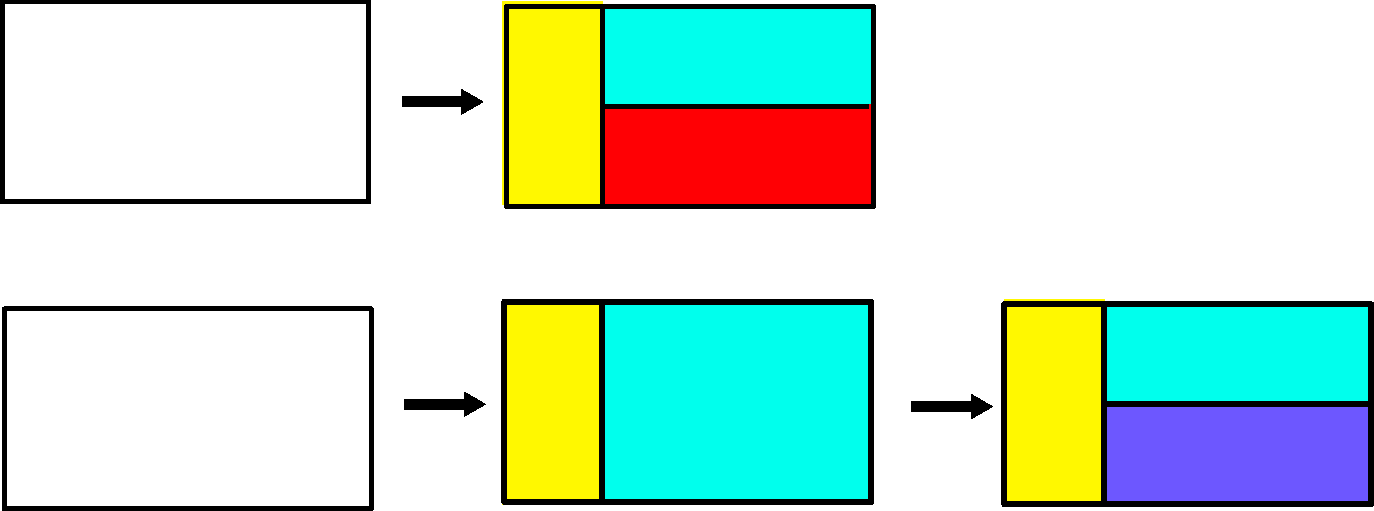
\includegraphics[width=0.8\columnwidth]{fig/tjunction.pdf}
\caption{%
\emph{Top:} Solving the labeling problem \eqref{eq:multicut_primal} with
more than two colors allows for T-junctions.
%
\emph{Bottom:} A sequence of two colorings can often model the same
T-junction. 
\label{fig:illustrate_t}}
\end{figure}





%%%%%%%%%%%%%%%%%%%%%%%%%%%%%%%%%%%%%%%%%%%%%%%%%%%%%%%%%%%%%%%
%                                                             %
%     THE CUT GLUE AND CUT AGLORITHM                          %
%                                                             %
%%%%%%%%%%%%%%%%%%%%%%%%%%%%%%%%%%%%%%%%%%%%%%%%%%%%%%%%%%%%%%%

\section{Cut, Glue \& Cut Algorithm\label{sec:cut_glue_cut_algorithm}}







%%%%%%%%%%%%%%%%%%%%%%%%%%%%%%%%%%%%%%%%%%%%%%%%%%%%%%%%%%%%%%%%%%%%%%%%%%%%%%%
% fig:illustration_cut
%%%%%%%%%%%%%%%%%%%%%%%%%%%%%%%%%%%%%%%%%%%%%%%%%%%%%%%%%%%%%%%%%%%%%%%%%%%%%%%
\begin{figure*}
\centering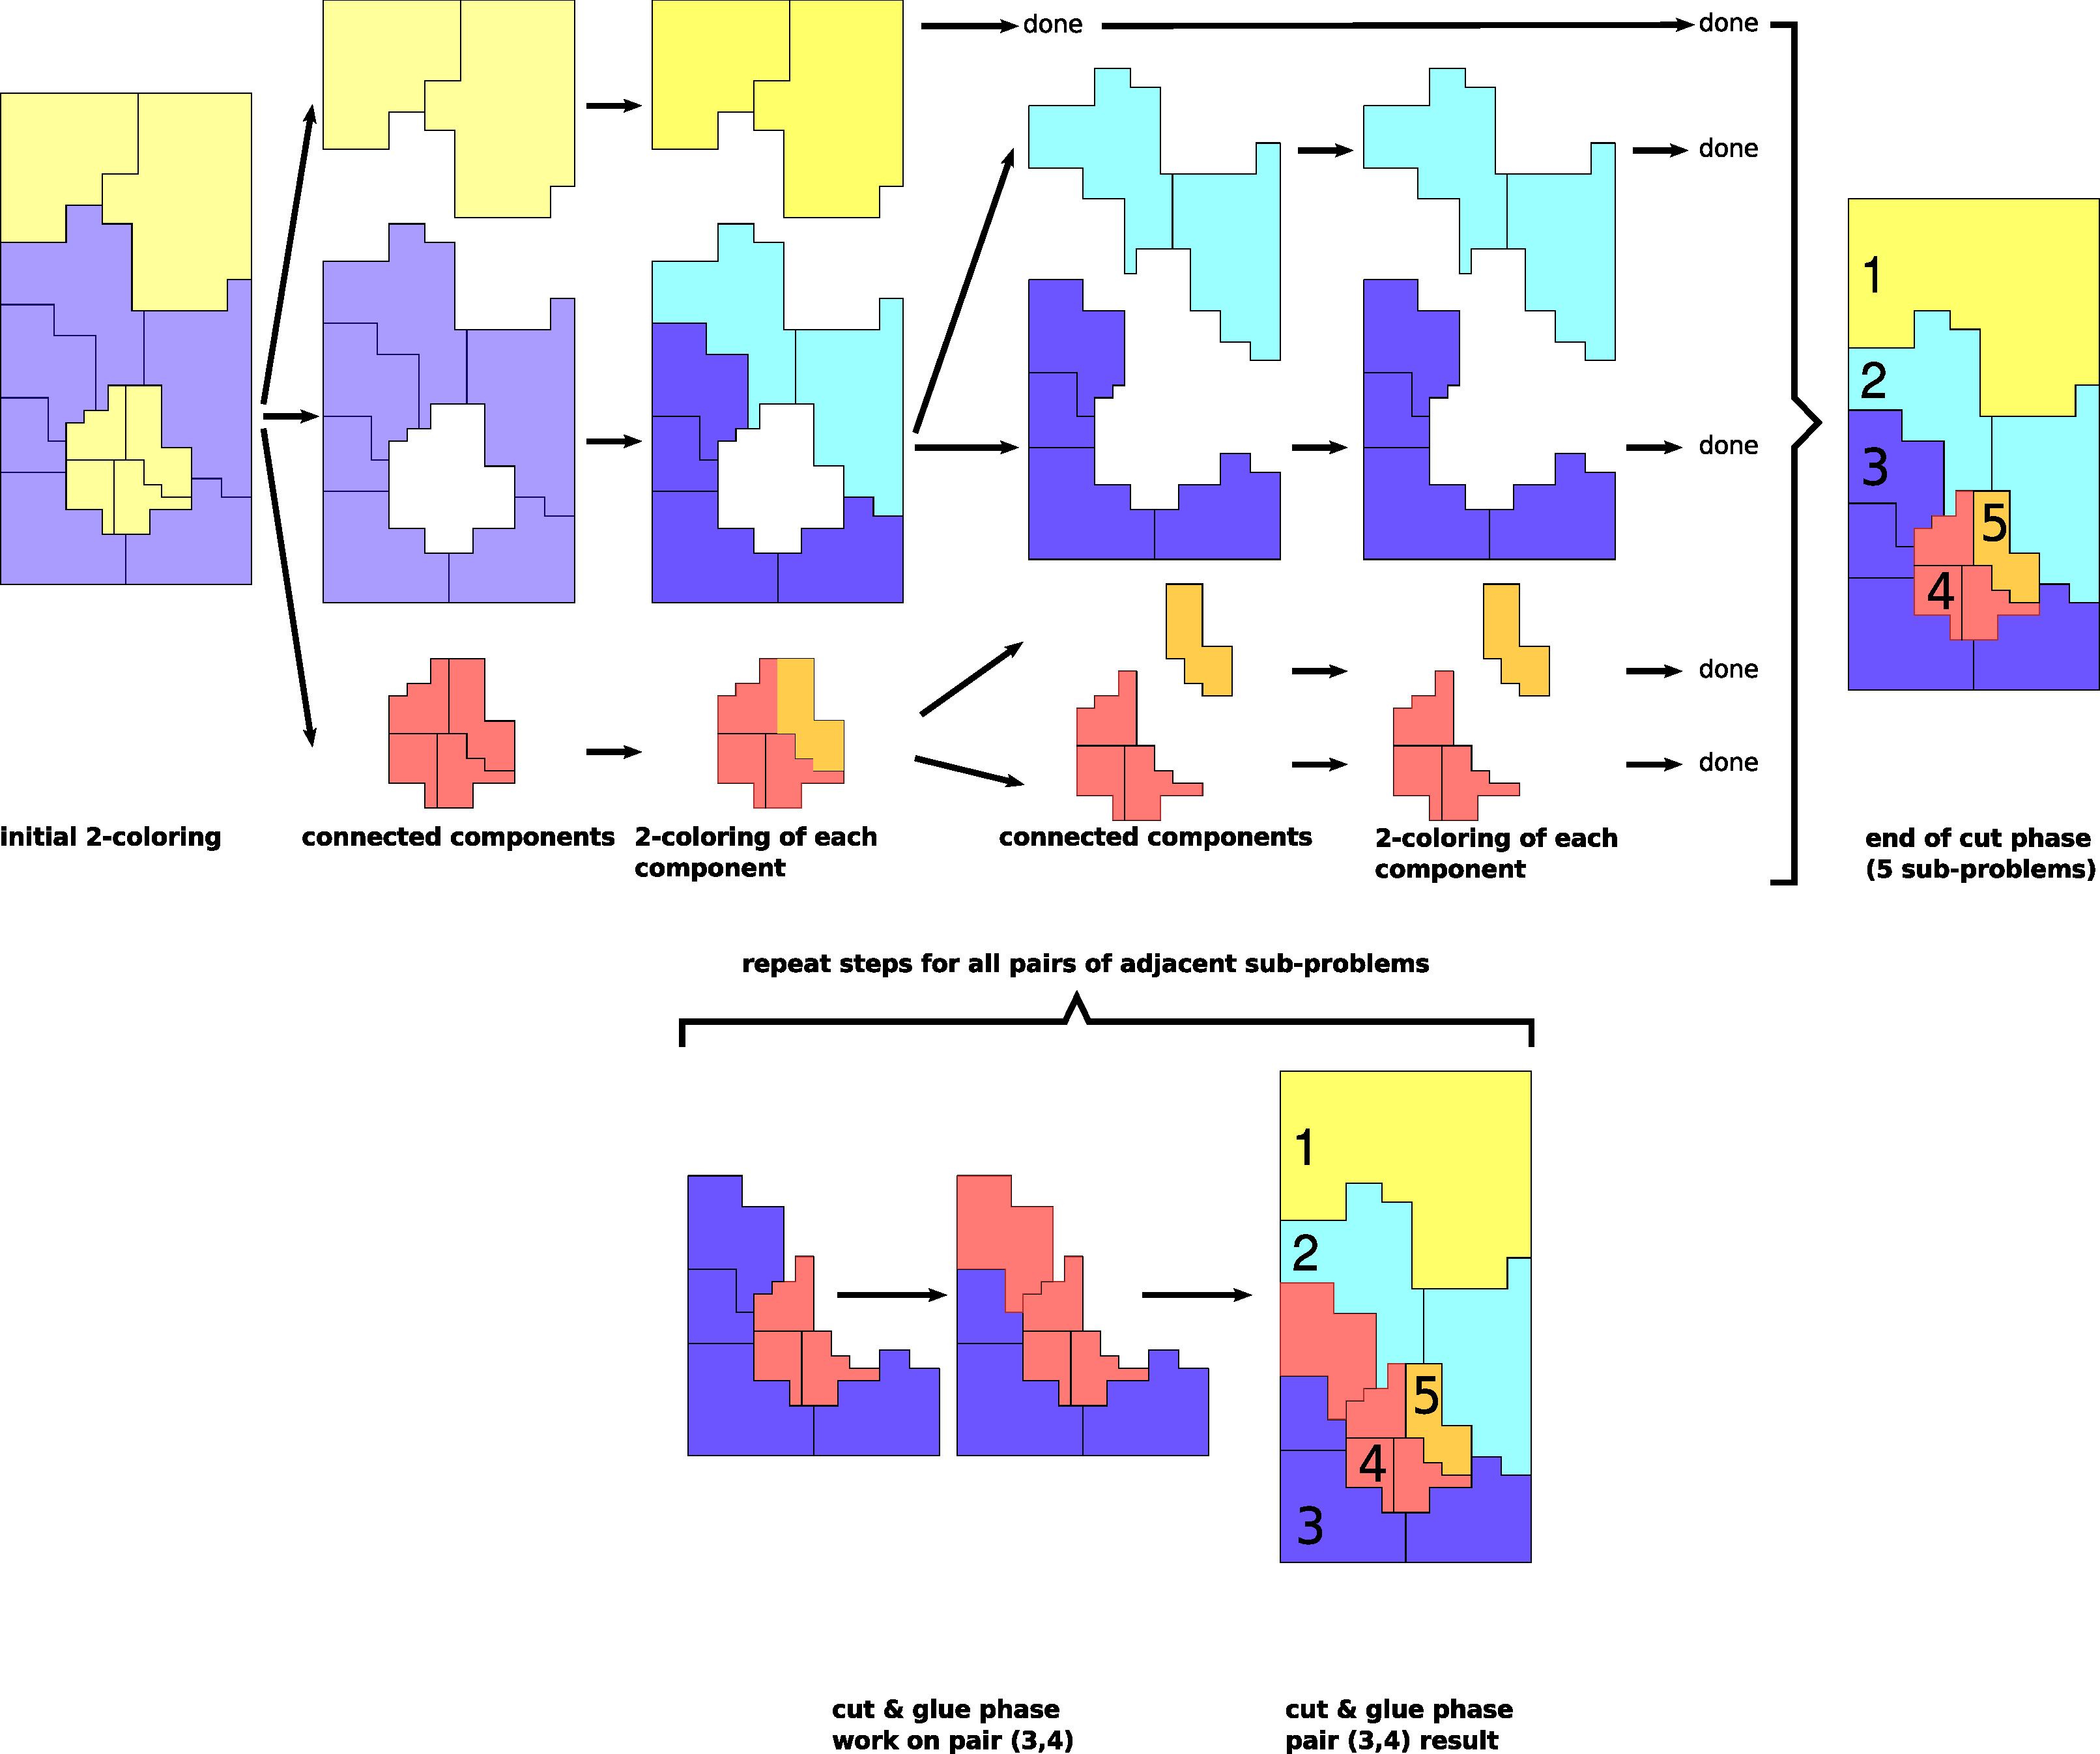
\includegraphics[width=\textwidth]{fig/illustration_new.pdf}
\caption{\label{fig:illustration_cut}%
%
\emph{Top}:
Illustration of the \emph{cut phase}.
The steps are visualized as a
%TODO bipartite
tree.
First, a weighted 2-coloring problem \eqref{eq:max_cut}
is solved on the initial
superpixel adjacency graph of an image. A connected-component labeling
yields the child nodes. For each node, the sequence of solving \eqref{eq:max_cut} 
and connected component labeling are repeated. Whenever a weighted 2-coloring
yields only a single component, the energy cannot be decreased any further and the
node has no children (``done'').
%
\emph{Bottom}:
Illustration of the \emph{glue\&cut phase}. In the illustrated move,
the regions labeled 3 and 4 are first merged and then a new, better 
partition is sought, which leads to a better global segmentation. This step
is repeated until no more improvement is possible.
}
\end{figure*}
%%%%%%%%%%%%%%%%%%%%%%%%%%%%%%%%%%%%%%%%%%%%%%%%%%%%%%%%%%%%%%%%%%%%%%%%%%%%%%%





\begin{algorithm}[t]
\ifx\DontPrintSemicolon\undefined
\else
\DontPrintSemicolon
\fi
\KwData{weighted graph $G\!=\!(V,E,\w)$}
\KwResult{approx. solution $Q$ to \eqref{eq:multicut_primal} for $G$}
%
$Q^0 \leftarrow $ segmentation of $G$ into positively connected components\;
\For{$n = 1\dots n_\text{iter}$}{
    $Q^n \leftarrow $ \text{cut\_phase}$(G, Q^{n-1})\quad\text{//Alg.~\ref{alg:cut_phase}}$\;
    $Q^n \leftarrow $ \text{glue\_cut\_phase}$(G, Q^{n})\quad\text{//Alg.~\ref{alg:glue_cut_phase}}$\;
    \If{$Q^n = Q^{n-1}$}{
        exit\;
    }
}
%
\caption{Cut, Glue \& Cut algorithm\label{alg:cut_glue_cut}}
\end{algorithm}

\paragraph{Overview}
The CGC algorithm (Alg.~\ref{alg:cut_glue_cut}) always maintains a valid partitioning of the graph, which
is iteratively improved by \emph{local} moves which
act on single or neighboring regions. It works
in two distinct phases:
\begin{inparaenum}[(i)]%
\item recursive \emph{cut phase} 
\item \emph{glue \& cut phase}%
\end{inparaenum}.

The cut phase recursively splits regions by
solving max-cut problems \eqref{eq:max_cut}, finally yielding a
finer, lower energy segmentation driven by the problem's weights.
In the glue \& cut
phase, any two neighboring segments are first merged and then a new cut is
sought between them by solving \eqref{eq:max_cut}.
These two phases are repeated and the process stops when the
energy cannot decrease any further.

\paragraph{Cut Phase}
In the \emph{cut phase}, the regions
are recursively split 
into smaller and smaller regions tuned to the weights $\w$ 
until a local optimum is found.
As \emph{cut moves} 
we consider the max-cut solution \eqref{eq:max_cut}
for a single given region $R$ to
find a better segmentation of the region
$\hat{y}\in\MC_{G_R}$,
and accept the
local move if the energy could be decreased compared
to the previous solution $\CUT_{G_R}(\y_R) = 0$.
%
The Partition Move Theorem then guarantees a
monotonically decreasing global energy for the segmentation.

The \emph{cut phase} is illustrated in the left
part of Fig.~\ref{fig:illustration_cut}, and is given as
Algorithm~\ref{alg:cut_phase}.
%
All regions are first inserted into a queue $Q$.
While $Q$ is not empty, take a region $R\;\in\;Q$,
then solve the max-cut problem \eqref{eq:max_cut} for $G_R$.
%If $G_R$ is planar, the solution can be found using the Blossom algorithm,
%otherwise an approximate solution is found by \mbox{QPBO-I}.
%
Finally, a connected component labeling of the solution defines a new set of
regions\footnote{%
Note that in general there may be more than two connected regions,
cf.~Fig.~\ref{fig:illustration_cut}, initial 2-coloring.
}.
%
If the suggested cut reduces the local energy, we add the induced regions
to $Q$.
%
Otherwise, the energy of region $R$ cannot further be reduced by this
type of move; region $R$ is marked as ``done'' and added to a list $Q'$.

\begin{algorithm}
\ifx\DontPrintSemicolon\undefined
\else
\DontPrintSemicolon
\fi
\KwData{weighted graph $G=(V,E,\w)$,
        segmentation into regions given as queue $Q$}
\KwResult{segmentation into smaller regions $Q'$}
%
$Q' \leftarrow \emptyset$\;
%
\While{$Q\neq\emptyset$}{
    $R \leftarrow \text{queue\_pop}(Q)$\;
    $\y_{E_R}$ $\leftarrow$ solve max-cut \eqref{eq:max_cut} for $G_R$\;
    \If{$\CUT_{G_R}(\y_{E_R}) < 0$}{
        $Q \leftarrow Q \cup \text{connected\_components}(\y_{E_R})$\;
    }
    \Else{
        $Q' \leftarrow Q' \cup R$
    }
}
\caption{Cut phase\label{alg:cut_phase}}
\end{algorithm}

\begin{algorithm}[t]
\ifx\DontPrintSemicolon\undefined
\else
\DontPrintSemicolon
\fi
\KwData{weighted graph $G\!=\!(V,E,\w)$, segmentation $Q$}
\KwResult{improved segmentation $Q$ wrt. \eqref{eq:multicut_primal}}
%
mark all edges $e\in E$ as dirty\;
$\bar{\y} \leftarrow \text{edge\_labeling}(Q)$\;
\While{true}{\label{alg:line:forever}%
    $c \leftarrow 0$\;
    $E' \leftarrow \{ e\in E\cap (R_1 \times R_2) | R_1,R_2\in Q\text{ adjacent}\}$\footnotemark\label{alg:line:e_dash}\;
    \For{$e=(i,j)\in E'$}{
        \If{$\bar{\y}_e=0$ or $e$ is clean}{
            continue\; 
        }
        find regions $R_1, R_2\!\in\!Q$, s.t. $i\in R_1$, $j\in R_2$\;
        $S \leftarrow R_1 \cup R_2\quad\text{//glue}$\;
        $\y_{E_S}$ $\leftarrow$ solve \eqref{eq:max_cut} for $G_S\quad\text{//cut}$\;
        {\color{blue}mark edges $E \cap S\times S$ clean$\quad(\star)$}\;
        \If{$\CUT_{G_S}(\y_{E_S}) < \CUT_{G_S}(\bar{\y}_{E_S})$}{
            $c \leftarrow c+1$\;
            {\color{blue}mark edges $E \cap S \times (V\setminus S)$ dirty$\quad(\star)$}\;
            $\text{CC} \leftarrow \text{connected\_components}(\y_{E_S})$\;
            {\color{blue}
            \If{$|\CC| > 2$}{
                mark edges $E \cap (S\times S)$ dirty$\quad(\star)$\;
            }}
            $Q \leftarrow Q\setminus \{R_1, R_2\} \cup \text{CC}$\;
            $\bar{\y} \leftarrow \text{edge\_labeling}(Q)$\;
        }
    }
    \If{$c = 0$}{
        break\label{alg:line:break}\;
    }
}
%
\caption{Glue \& Cut phase\label{alg:glue_cut_phase}}
\end{algorithm}
\footnotetext{Note that by using $E'$ instead of $E$, we consider only
one representative edge for each boundary between two regions for
performance reasons.}%

\paragraph{Glue \& Cut Phase}
In this phase, we consider \emph{Glue \& Cut moves}
of pairs of adjacent segments until the energy cannot be decreased any further,
yielding a better solution.

Intuitively, we expect that two common local operations can decrease the
energy: (i) merging two segments or (ii) moving the boundary between
two adjacent segments. This motivates our algorithm:

We again apply the Partition Move Theorem from Sec.~\ref{sec:cut_moves}.
Given two adjacent regions $R_1, R_2$ in the current segmentation,
we consider the \emph{merged region} $R = R_1 \cup R_2$ (\emph{glue}),
and find a new segmentation $\hat{\y}\in\MC_{G_R}$ (\emph{cut})
by solving the max-cut problem \eqref{eq:max_cut}.
%either
%to optimality if $G_R$ is planar, or using \mbox{QPBO-I} else.
The local move is accepted if the energy $\CUT_{G_R}(\hat{\y})$
is lower than the energy of the previous cut.
The Partition Move Theorem then guarantees a
monotonically decreasing energy for the segmentation.

Formally,
(Alg.~\ref{alg:glue_cut_phase} and Fig.~\ref{fig:illustration_cut}, right),
the glue \& cut phase starts from a given segmentation $Q$.
We first obtain its edge labeling $\bar{\y}$.
Initially, all edges $e\in E$ are marked ``dirty''.
%
The following is repeated (line \ref{alg:line:forever}):
%
For each pair $(R_1, R_2)$ of adjacent regions
we pick a single representative edge from the shared boundary 
$E\cap(R_1\times R_2)$ to form the set $E'$ (line \ref{alg:line:e_dash}). 
Then, for each such representative $e=(i,j)$ with $\y_e=1$ and which
is marked dirty, we find the best glue \& cut move as described above.
If, after processing all $e\in E'$, no move could be performed, we break
out of the outer loop (line \ref{alg:line:break}).

\paragraph{Book-keeping of modified boundaries.}
In order to avoid re-solving the same problem multiple times, the algorithm
marks edges as ``dirty'' or ``clean''. If two adjacent regions are only separated
by clean edges, a glue \& cut move is \emph{not} considered for this pair.
%
In Alg.~\ref{alg:glue_cut_phase}, statements related to book-keeping
are marked with $(\star)$.

Imagine an accepted glue \& cut move which yields exactly two regions
$R_1$ and $R_2$.
We mark the boundary between $R_1$ and $R_2$, $E\cap(R_1\times R_2)$, as clean,
since re-solving \eqref{eq:max_cut} for $R_1\cup R_2$
would again lead to the same two-coloring into $R_1$ and $R_2$.
%
However, if an adjacent pair $(R_1, R_3)$ is chosen subsequently, 
a glue \& cut move could alter
region $R_1$ into $R_1'$.
Therefore, a move between $R_1'$ and $R_2$ could improve the energy again.
To allow this move it is necessary to 
mark the boundary of $R_1' \cup R_2$ as dirty.
%
Note that for the case where an accepted move yields \emph{more than two regions},
the above would not be correct and the internal edges have to be marked dirty.
%
%Because there are more than one pair of adjacent
%regions generated. We need to consider each such pair \emph{separately}, 
%necessitating to set all of them dirty.




%%%%%%%%%%%%%%%%%%%%%%%%%%%%%%%%%%%%%%%%%%%%%%%%%%%%%%%%%%%%%%%
%                                                             %
%     EXPERIMENTS                                             %
%                                                             %
%%%%%%%%%%%%%%%%%%%%%%%%%%%%%%%%%%%%%%%%%%%%%%%%%%%%%%%%%%%%%%%


\iffalse
\begin{figure*}
\centering
\subfloat[original image]{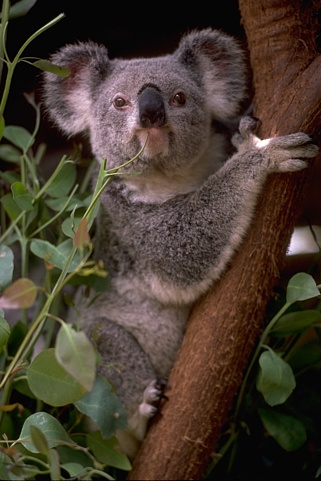
\includegraphics[width=0.17\textwidth]{%
fig/visualcompare/69015.jpg%
}}~%
\subfloat[superpixels]{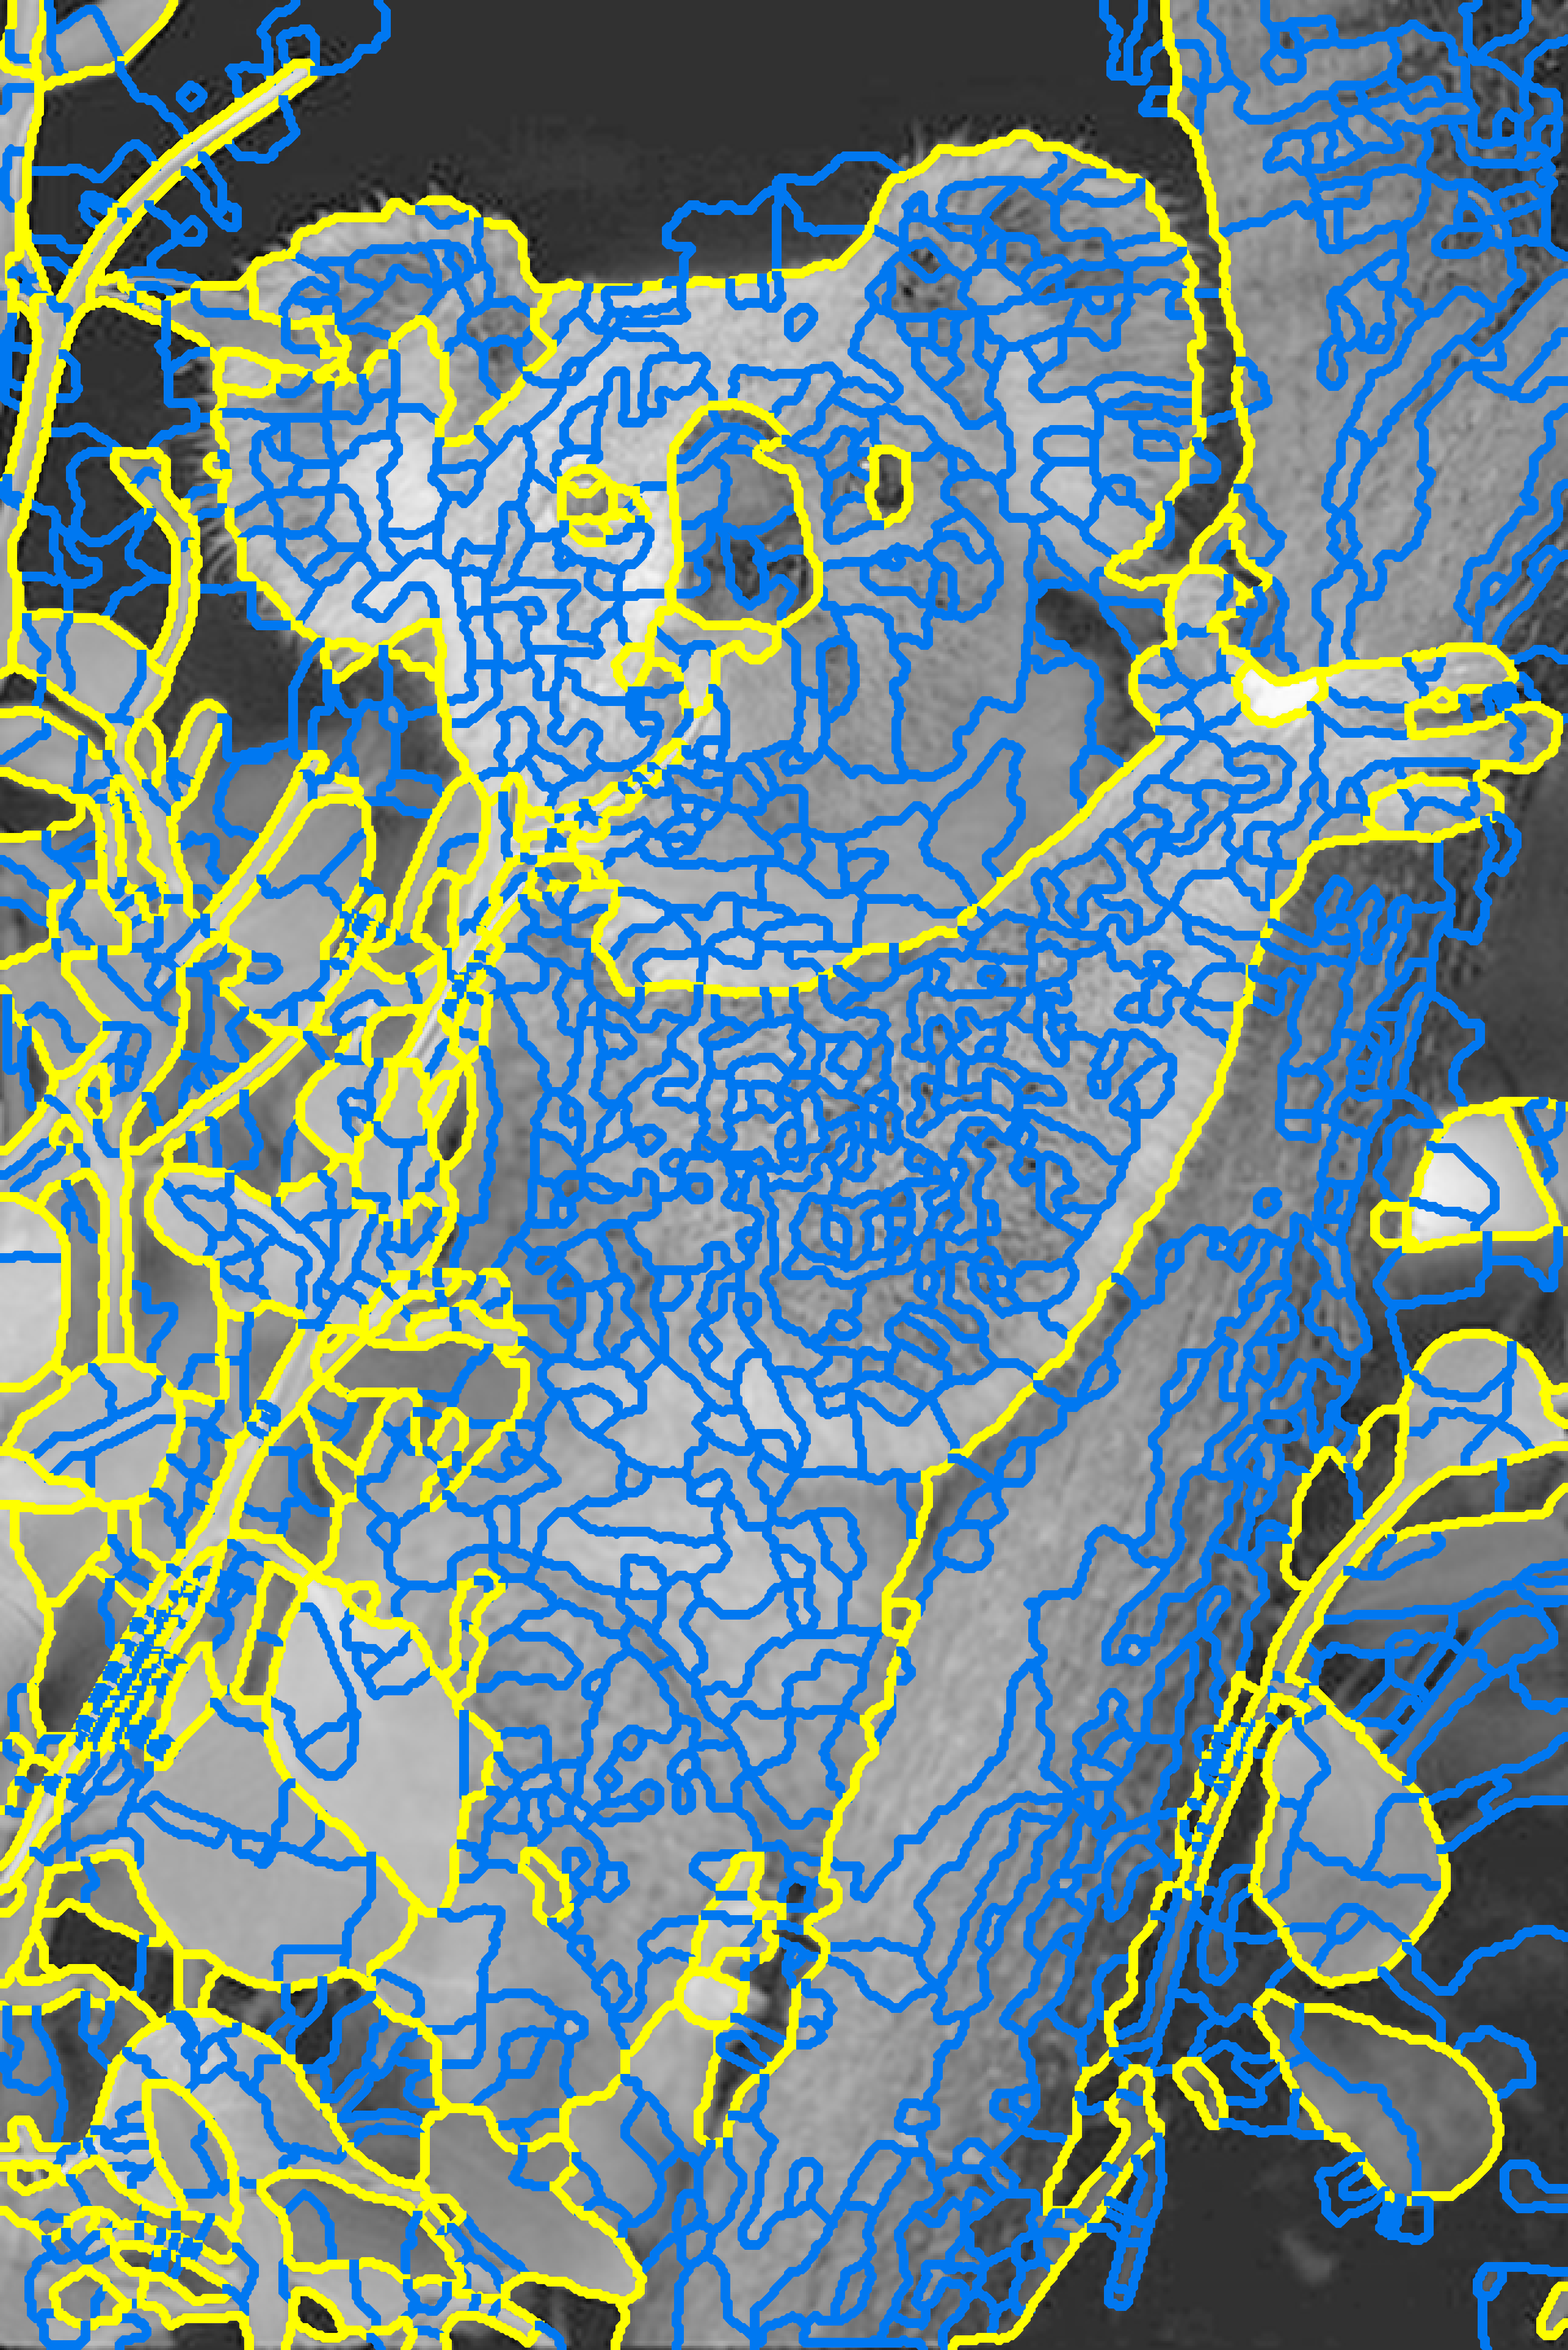
\includegraphics[width=0.17\textwidth]{%
fig/visualcompare/69015_superpixel.png%
}}~%
\subfloat[first two coloring]{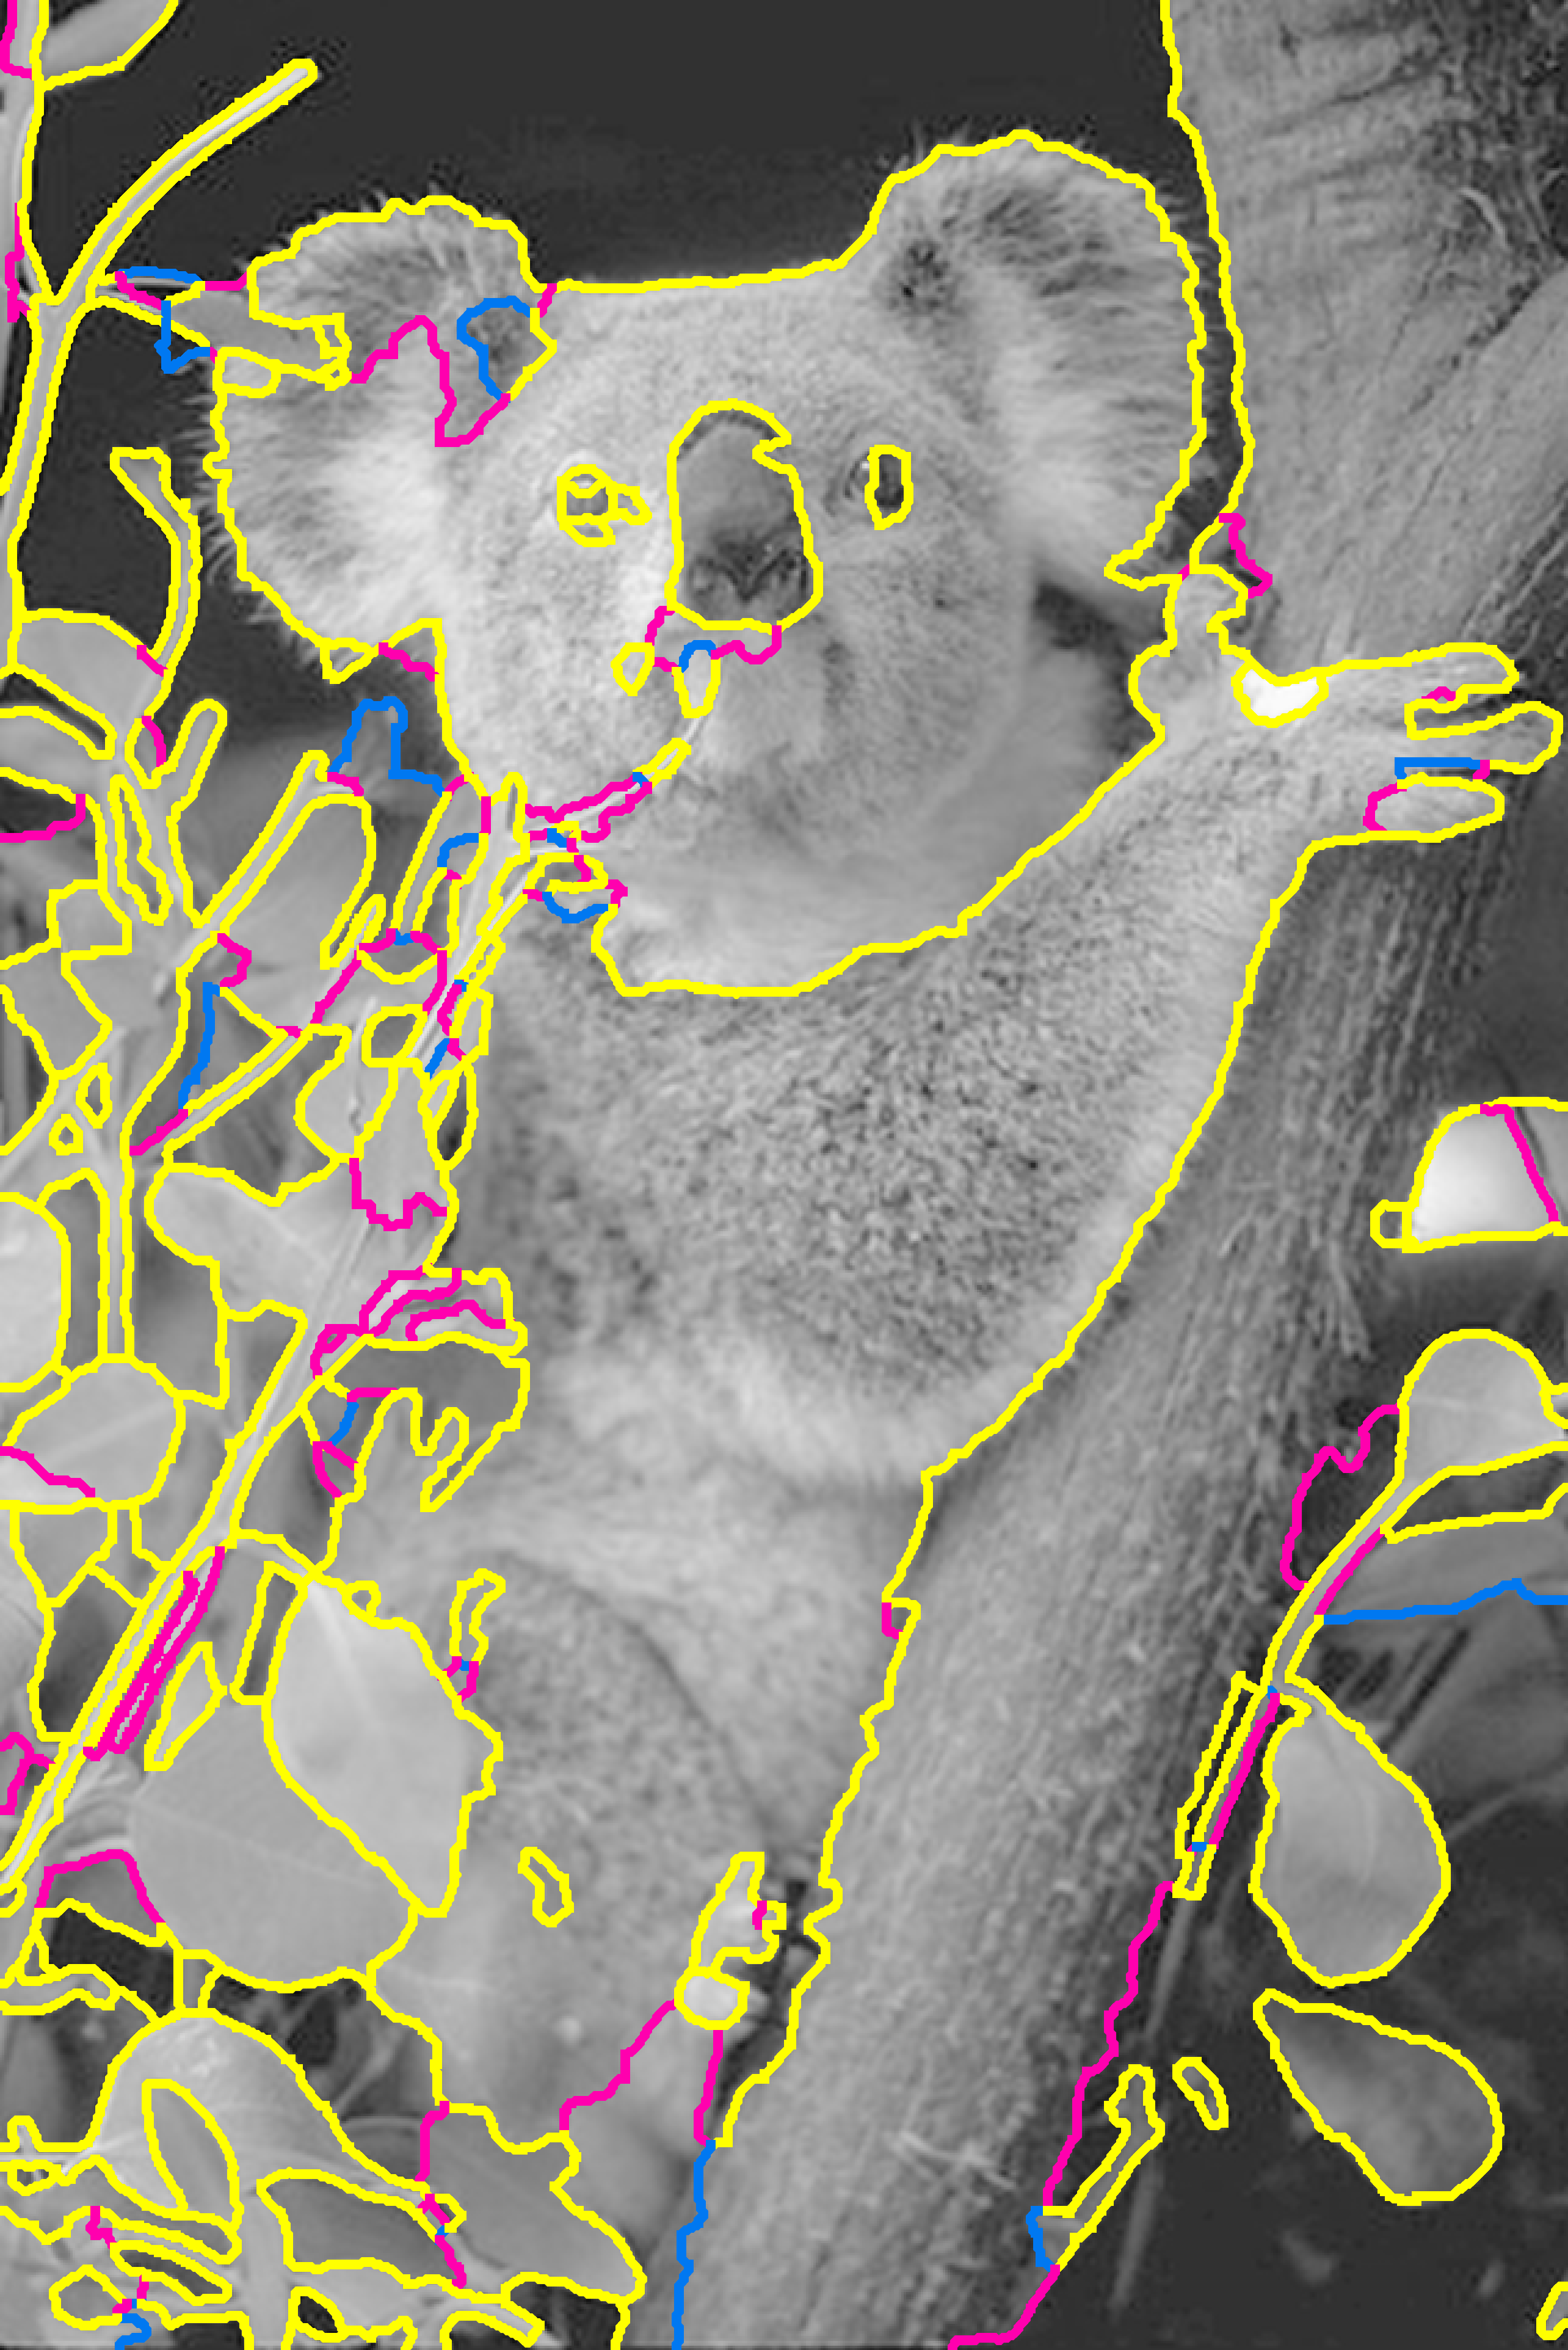
\includegraphics[width=0.17\textwidth]{%
fig/visualcompare/69015_CGC_cut_phase_00.png%
}}~%
\subfloat[end of cut phase]{%
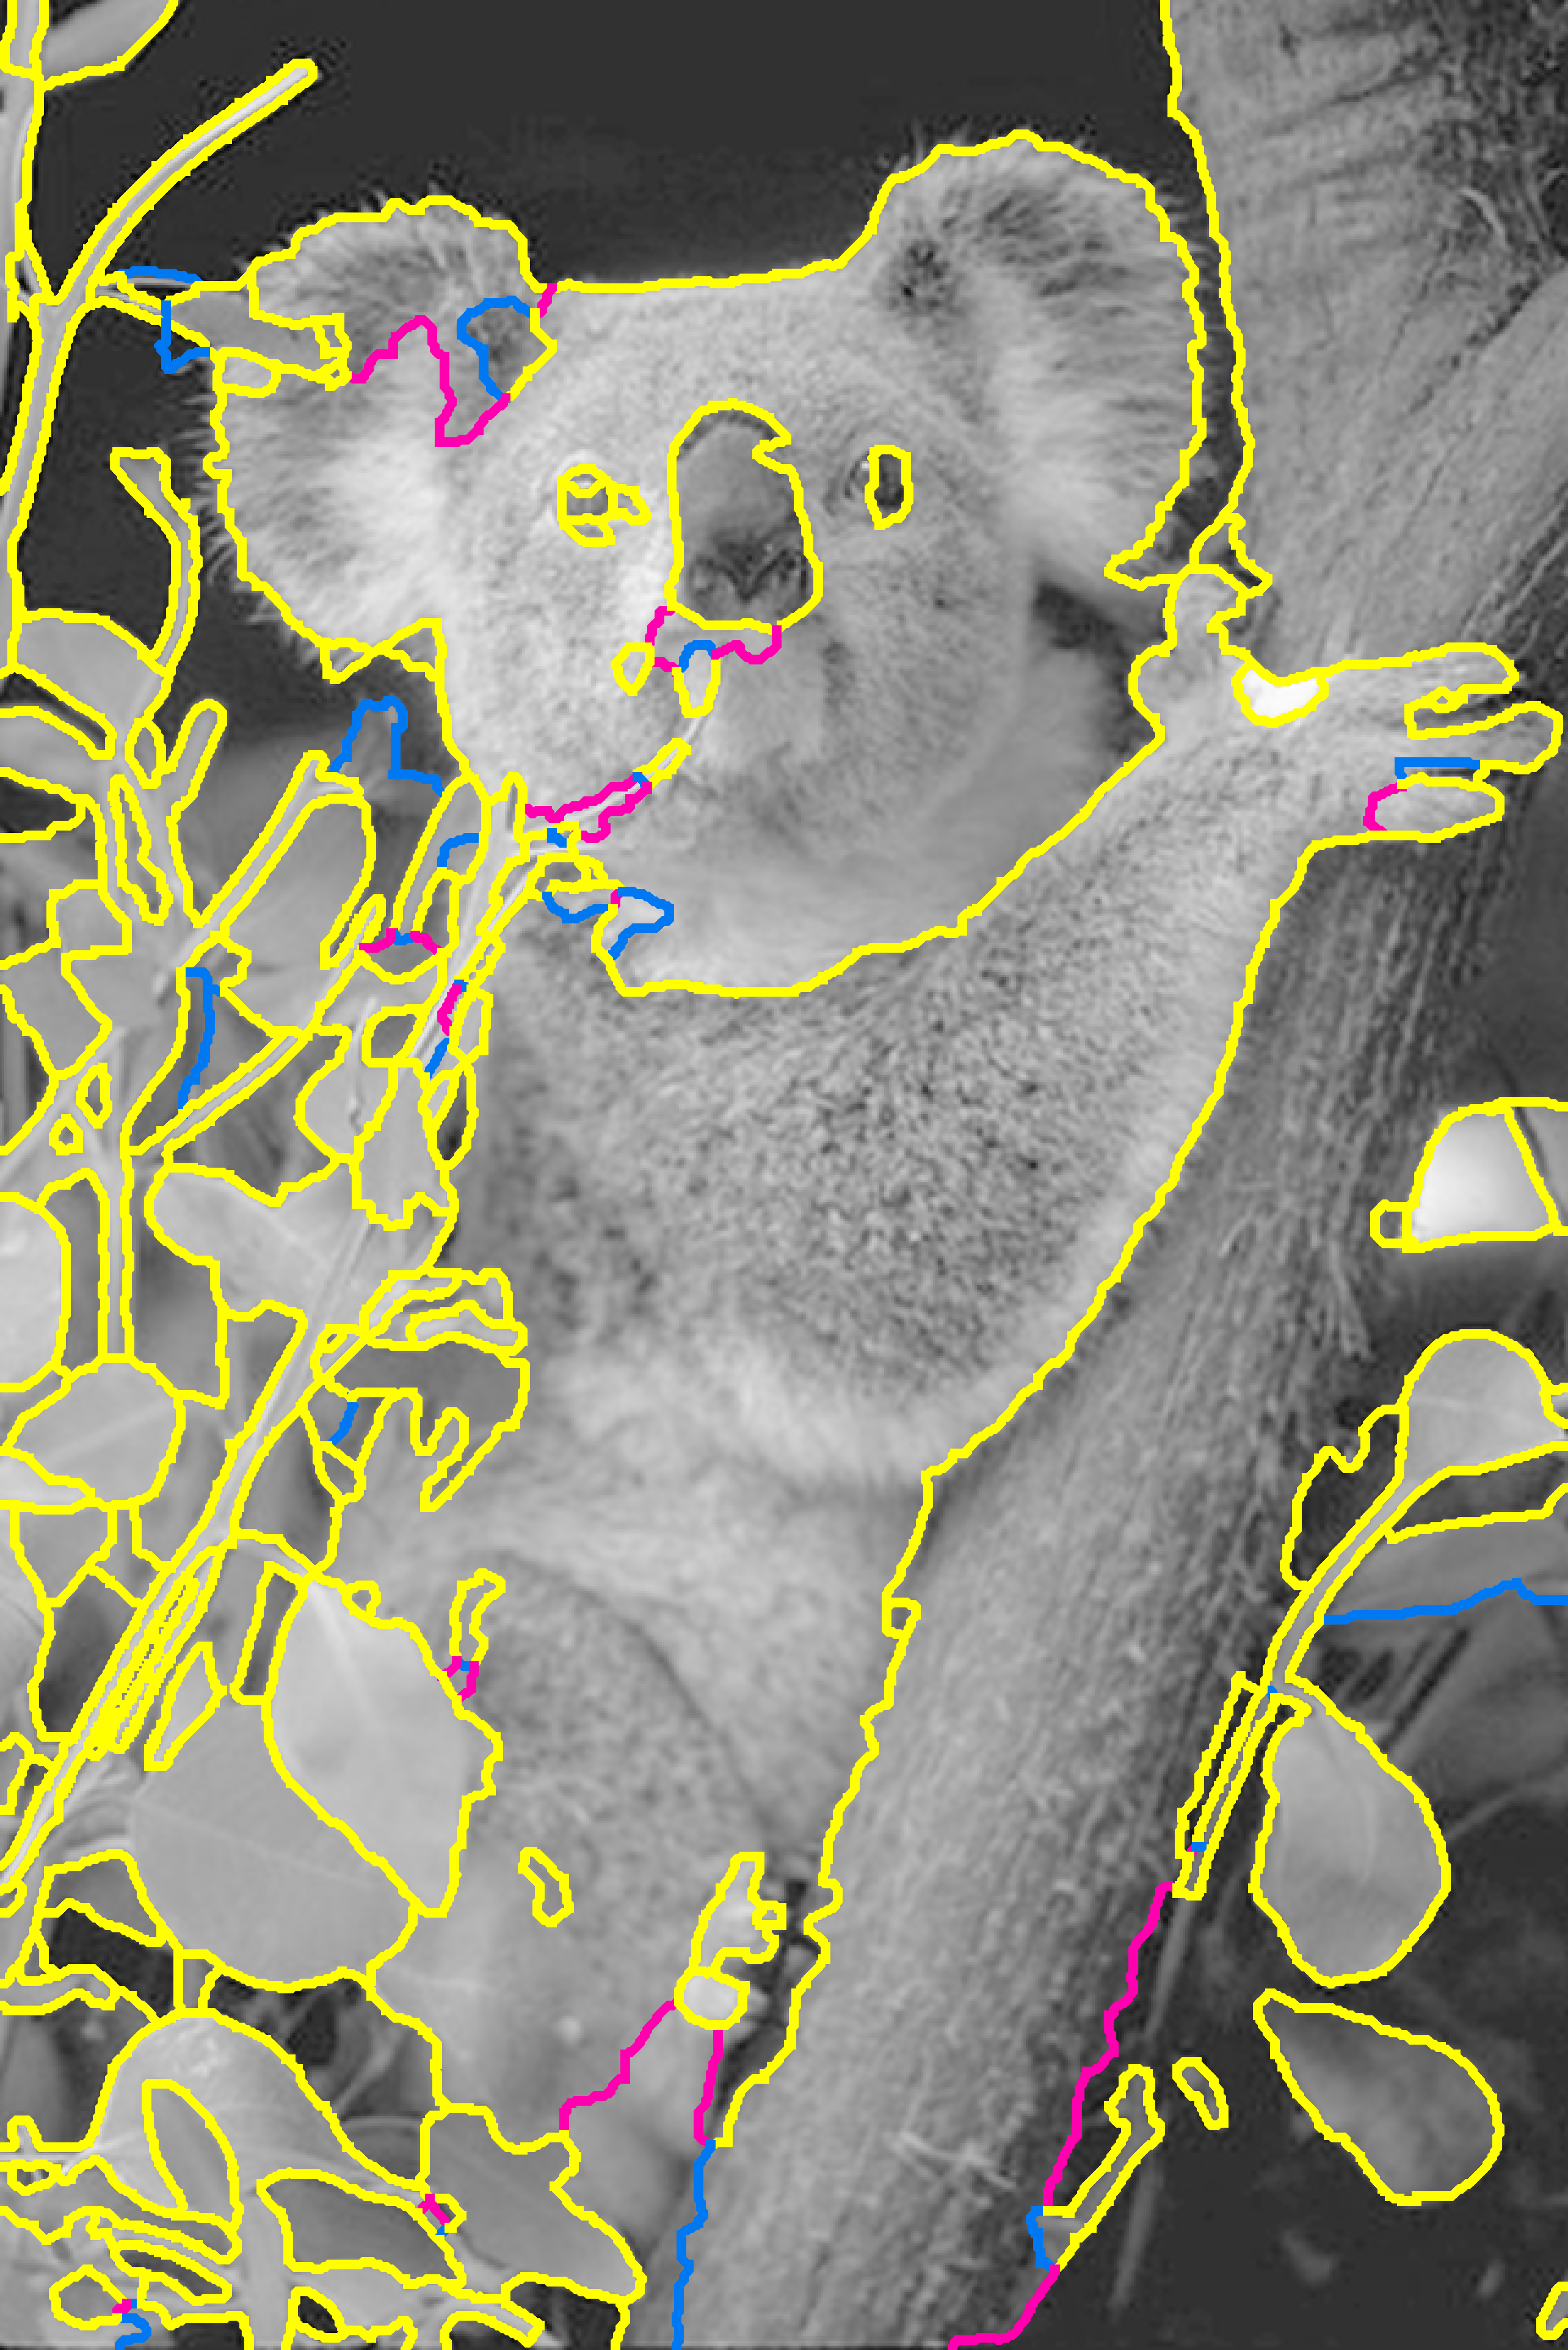
\includegraphics[width=0.17\textwidth]{%
fig/visualcompare/69015_CGC_cut_phase_20.png%
}}~%
\subfloat[CGC]{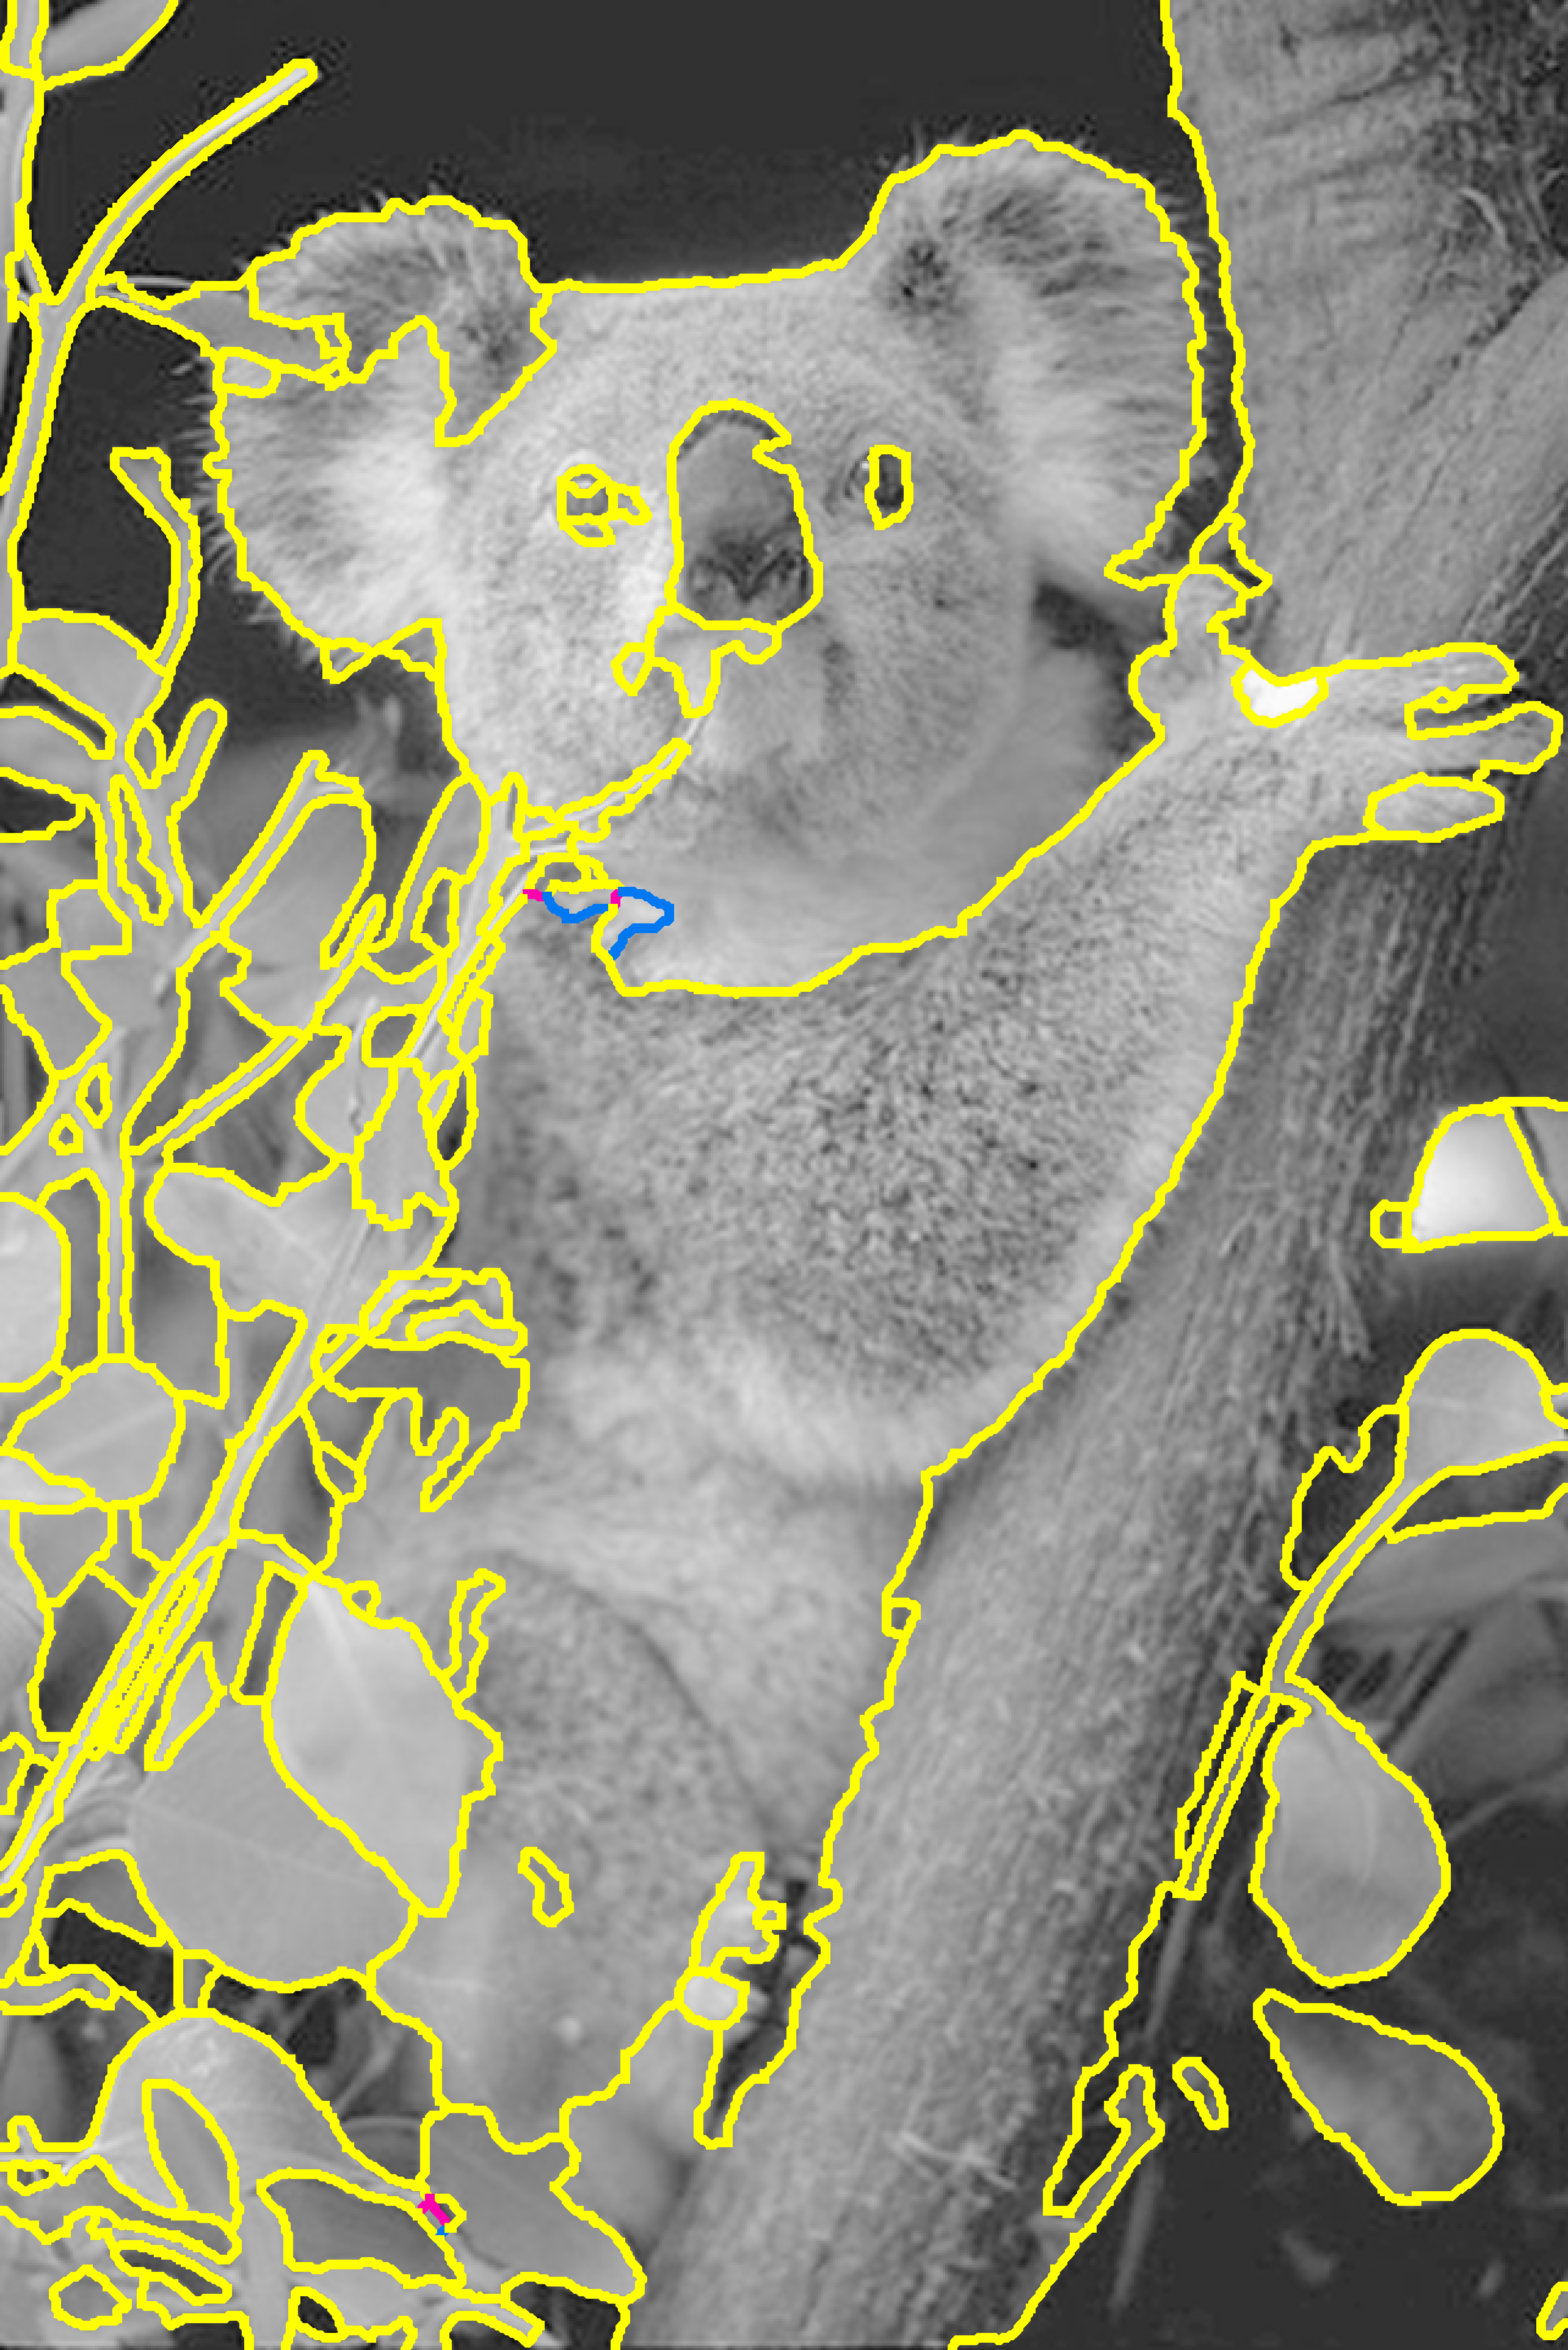
\includegraphics[width=0.17\textwidth]{%
fig/visualcompare/69015_CGC.png%
}}\\%
%
\subfloat[MC-I (global opt.)]{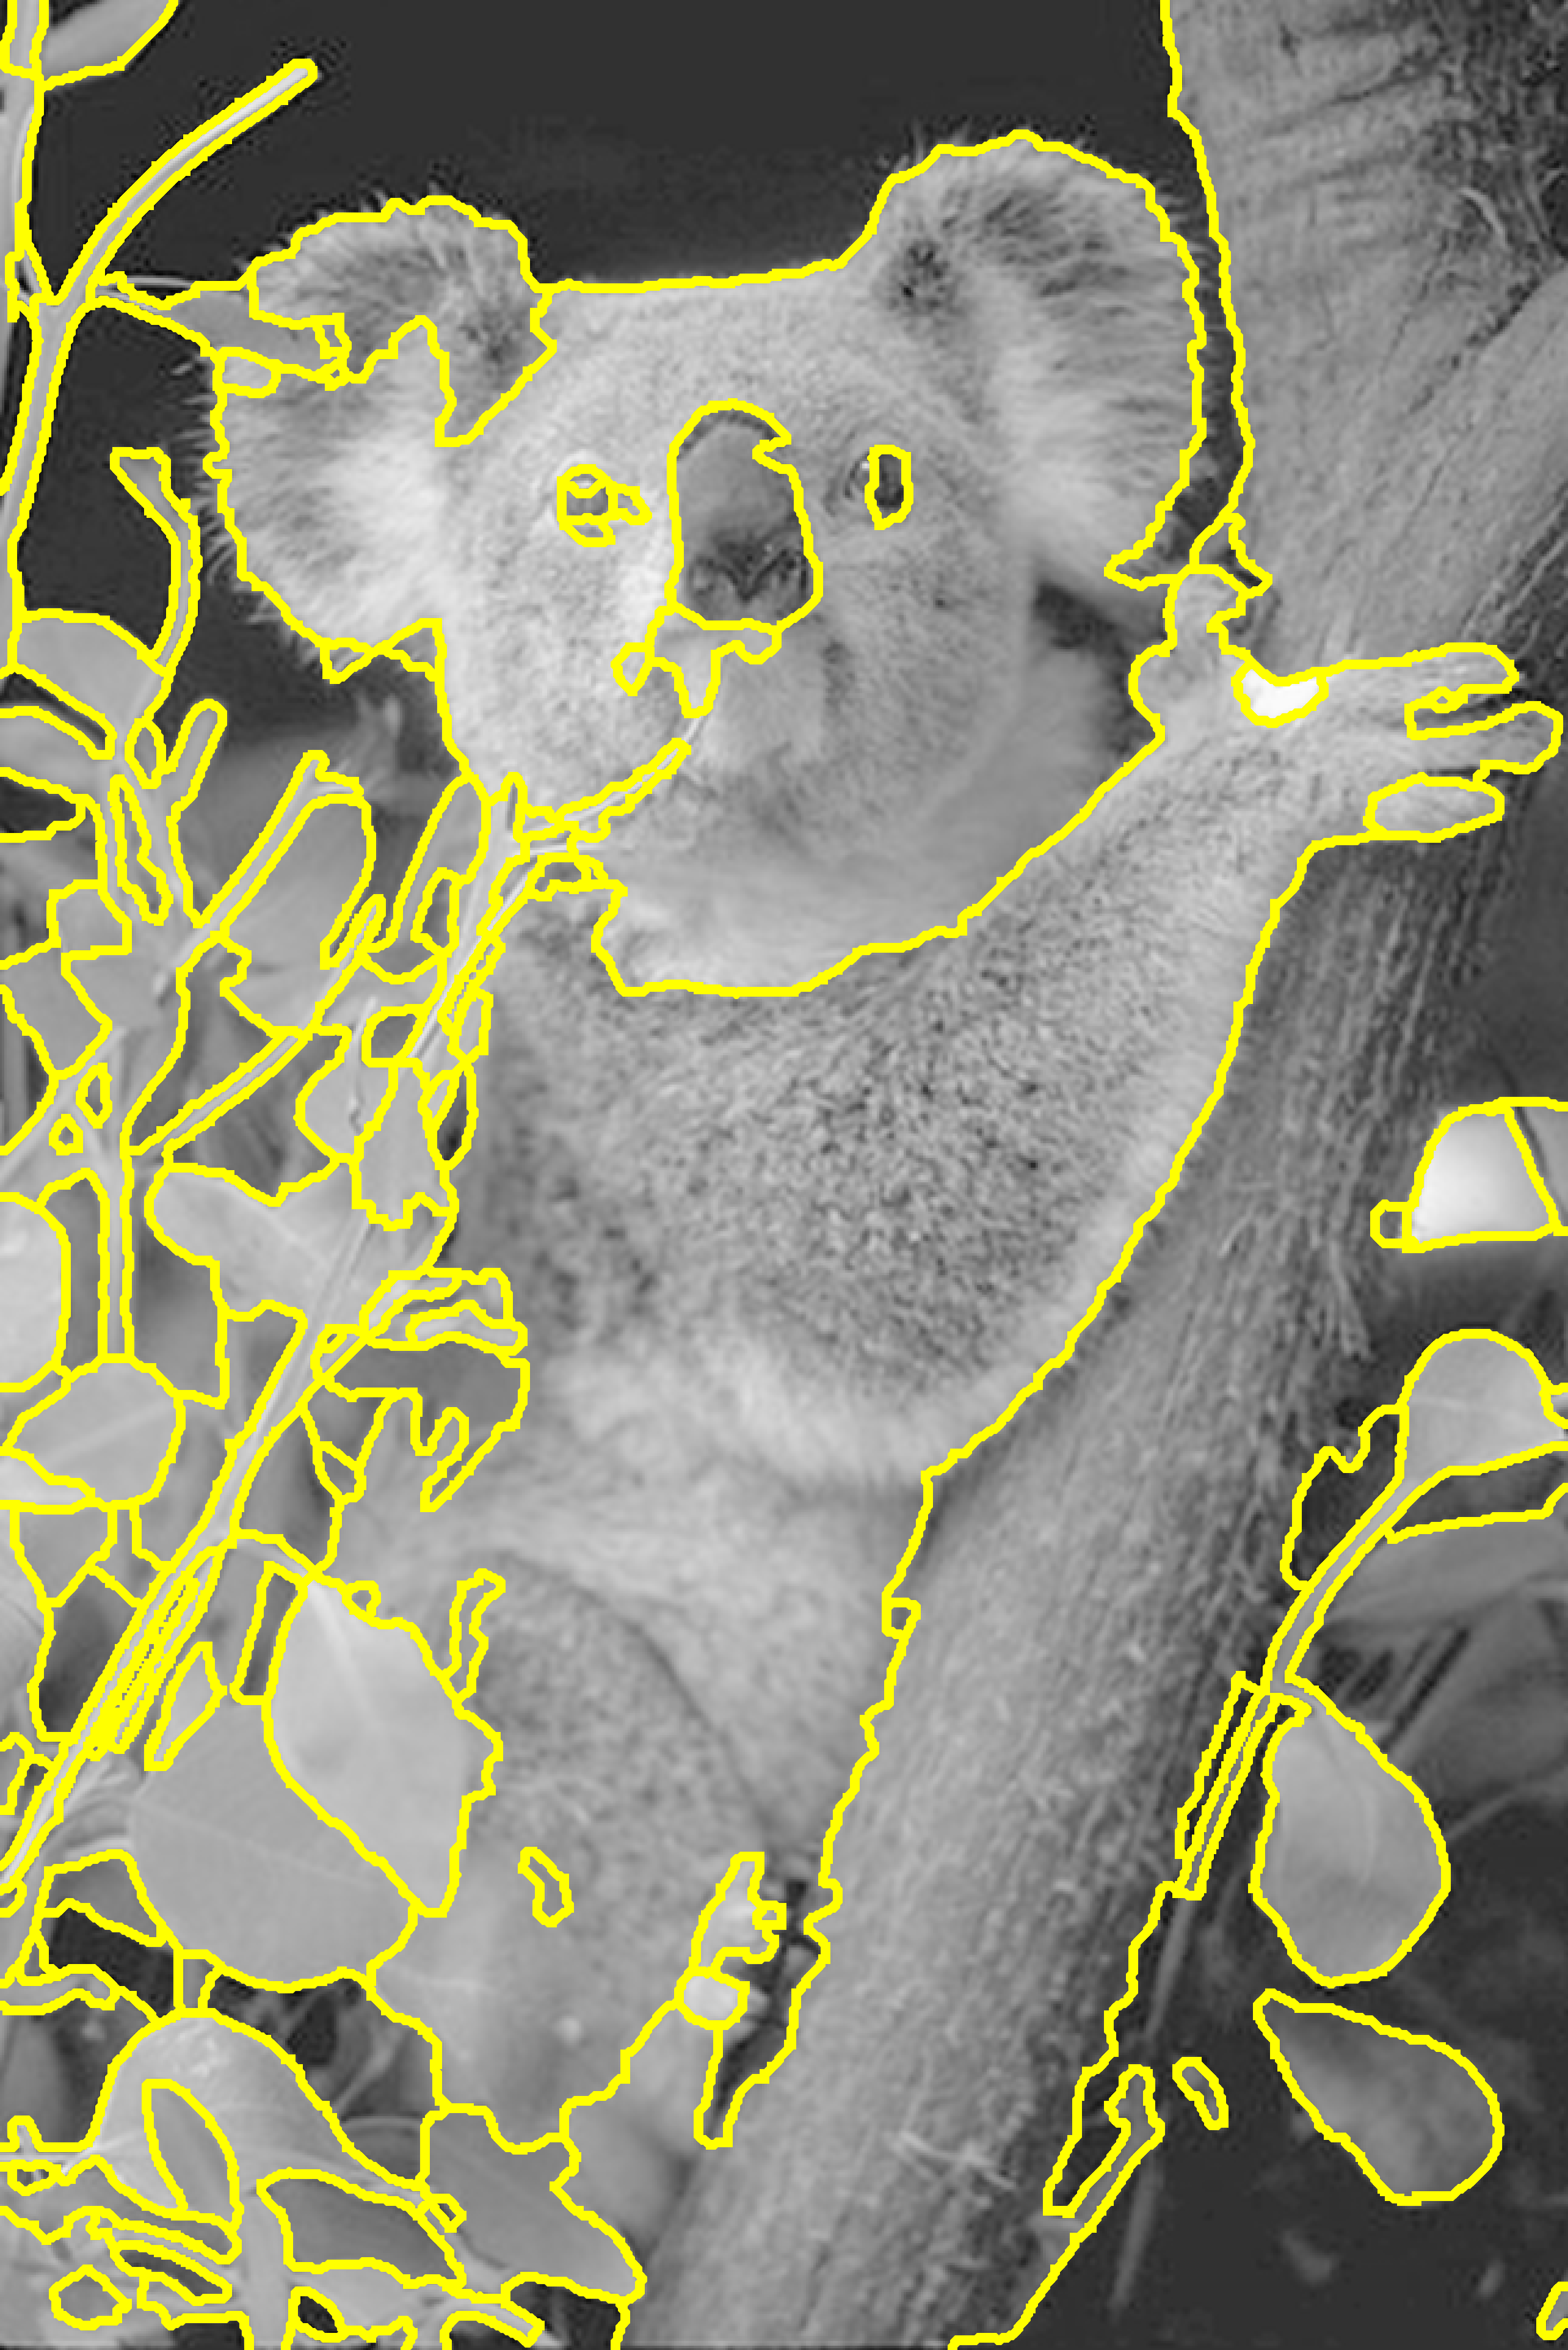
\includegraphics[width=0.17\textwidth]{%
fig/visualcompare/69015_MCI.png%
}}~%
\subfloat[MC-R]{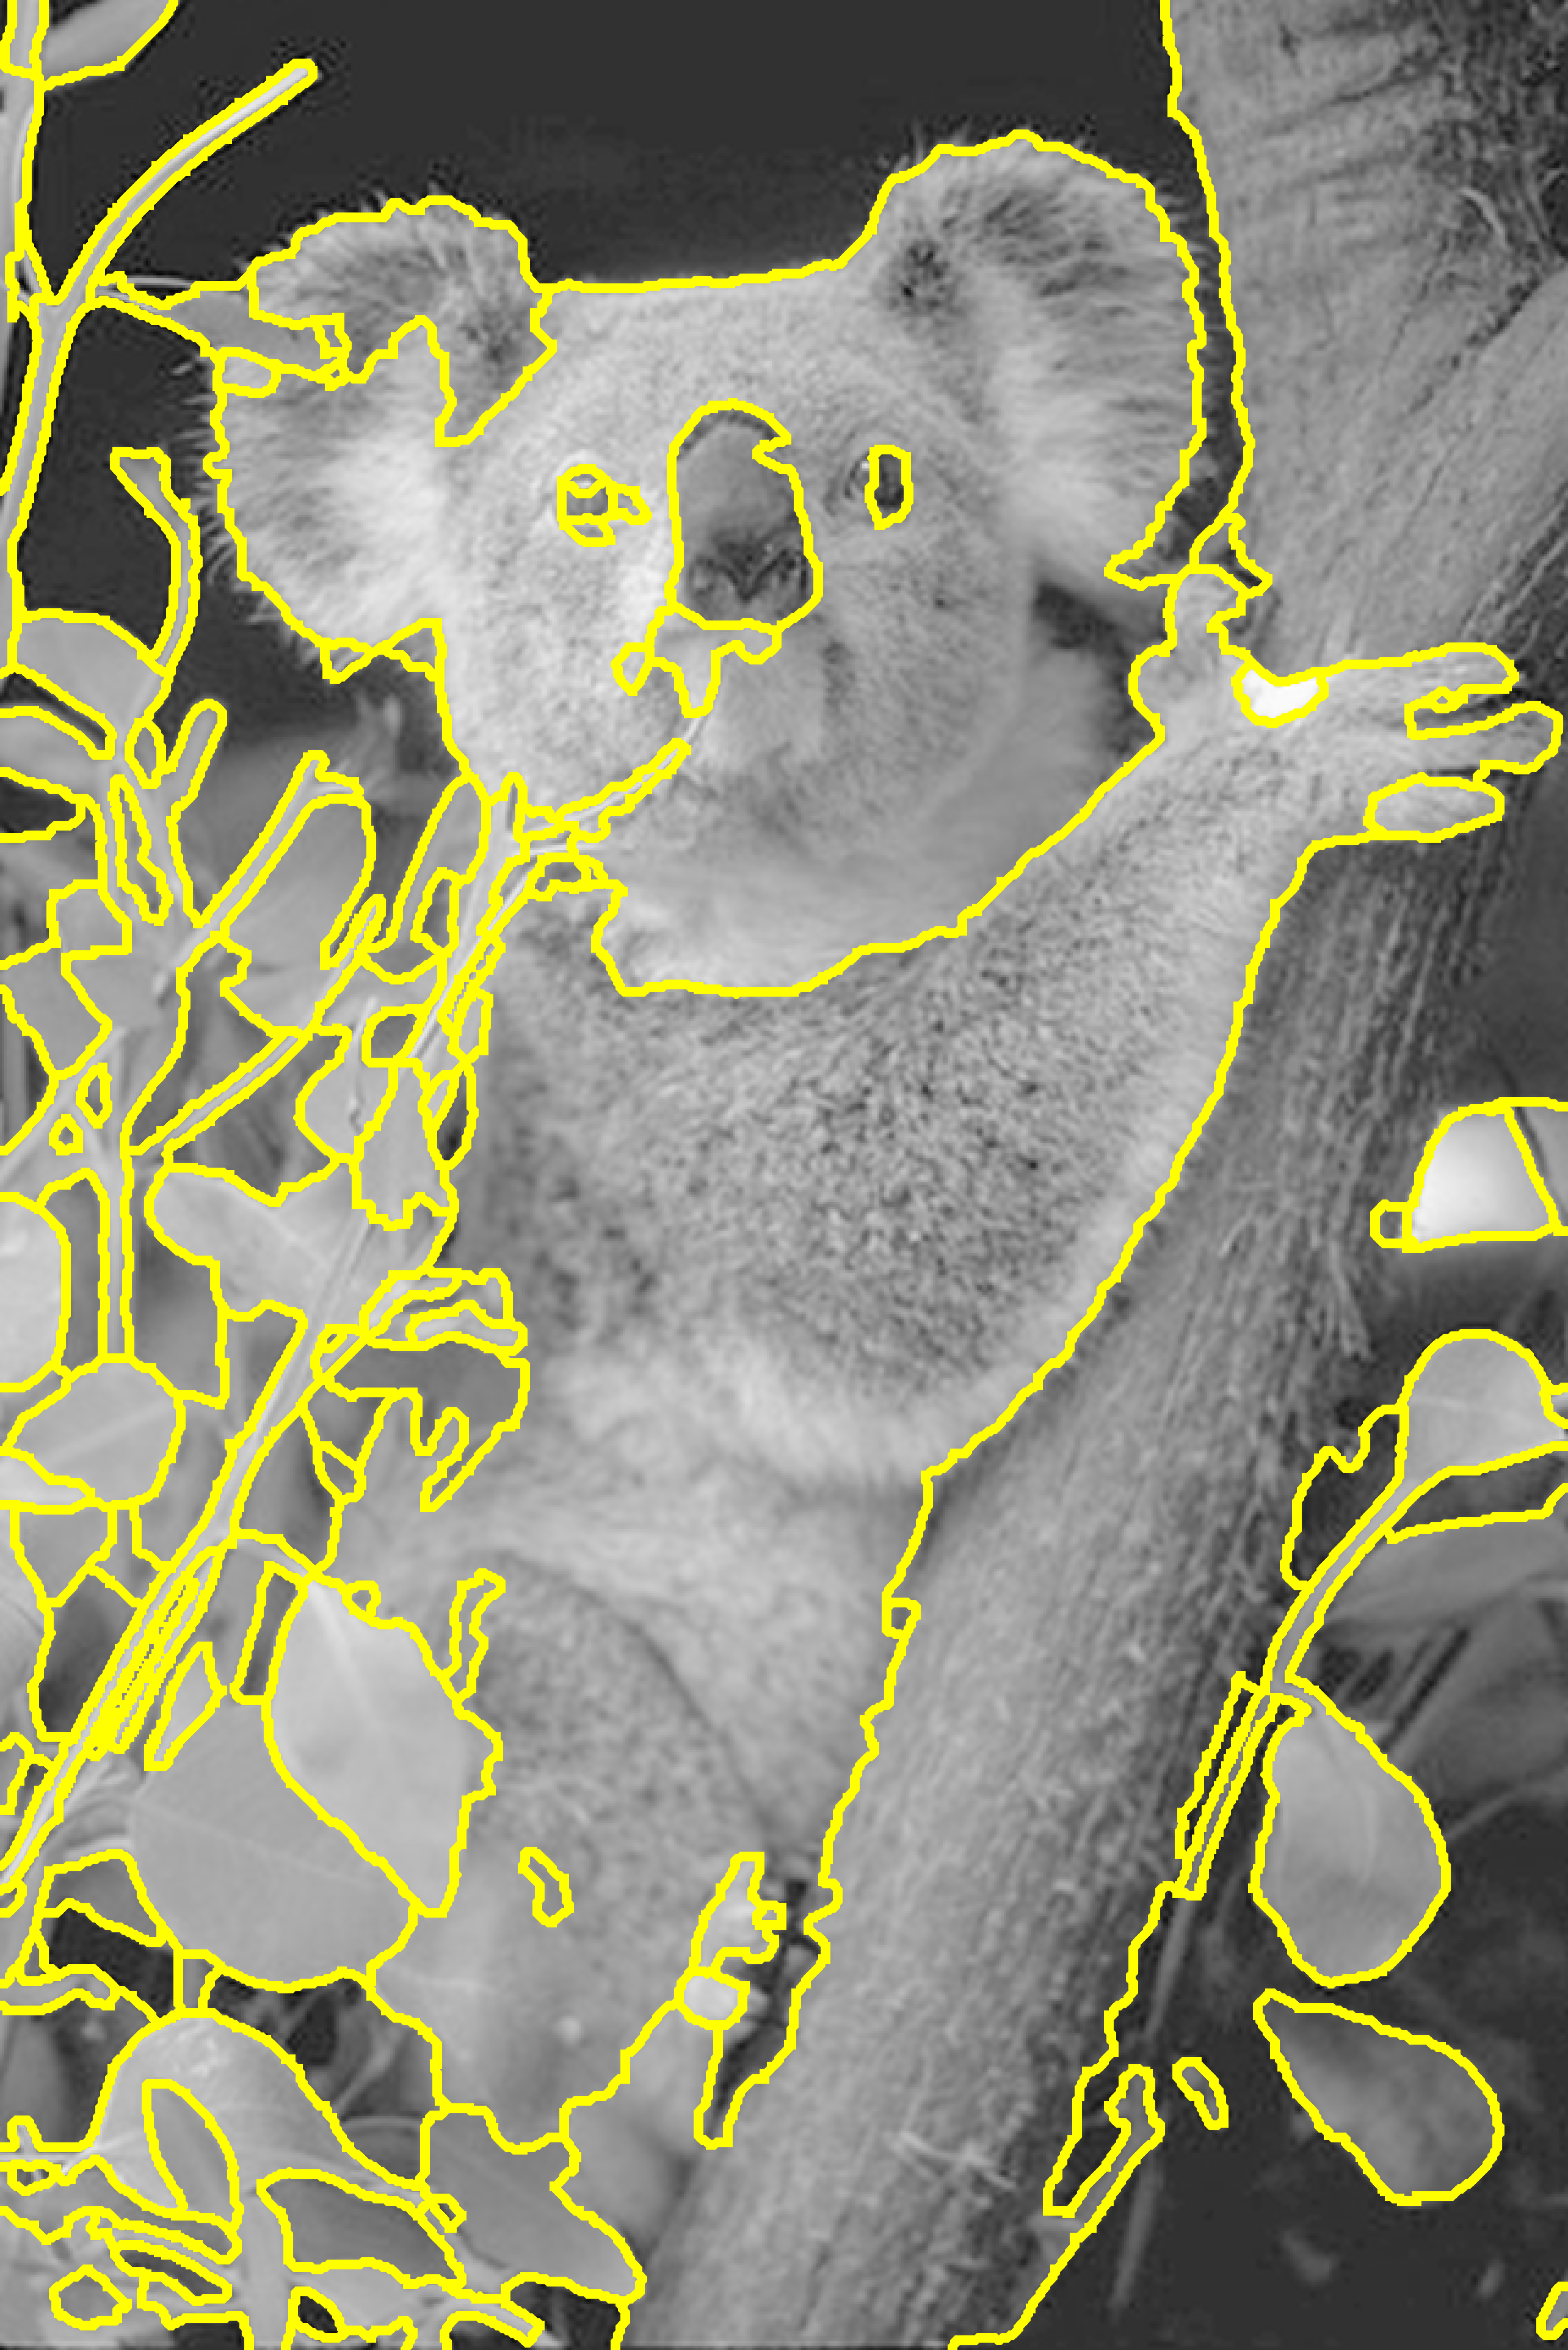
\includegraphics[width=0.17\textwidth]{%
fig/visualcompare/69015_MCR.png%
}}~%
\subfloat[PlanarCC]{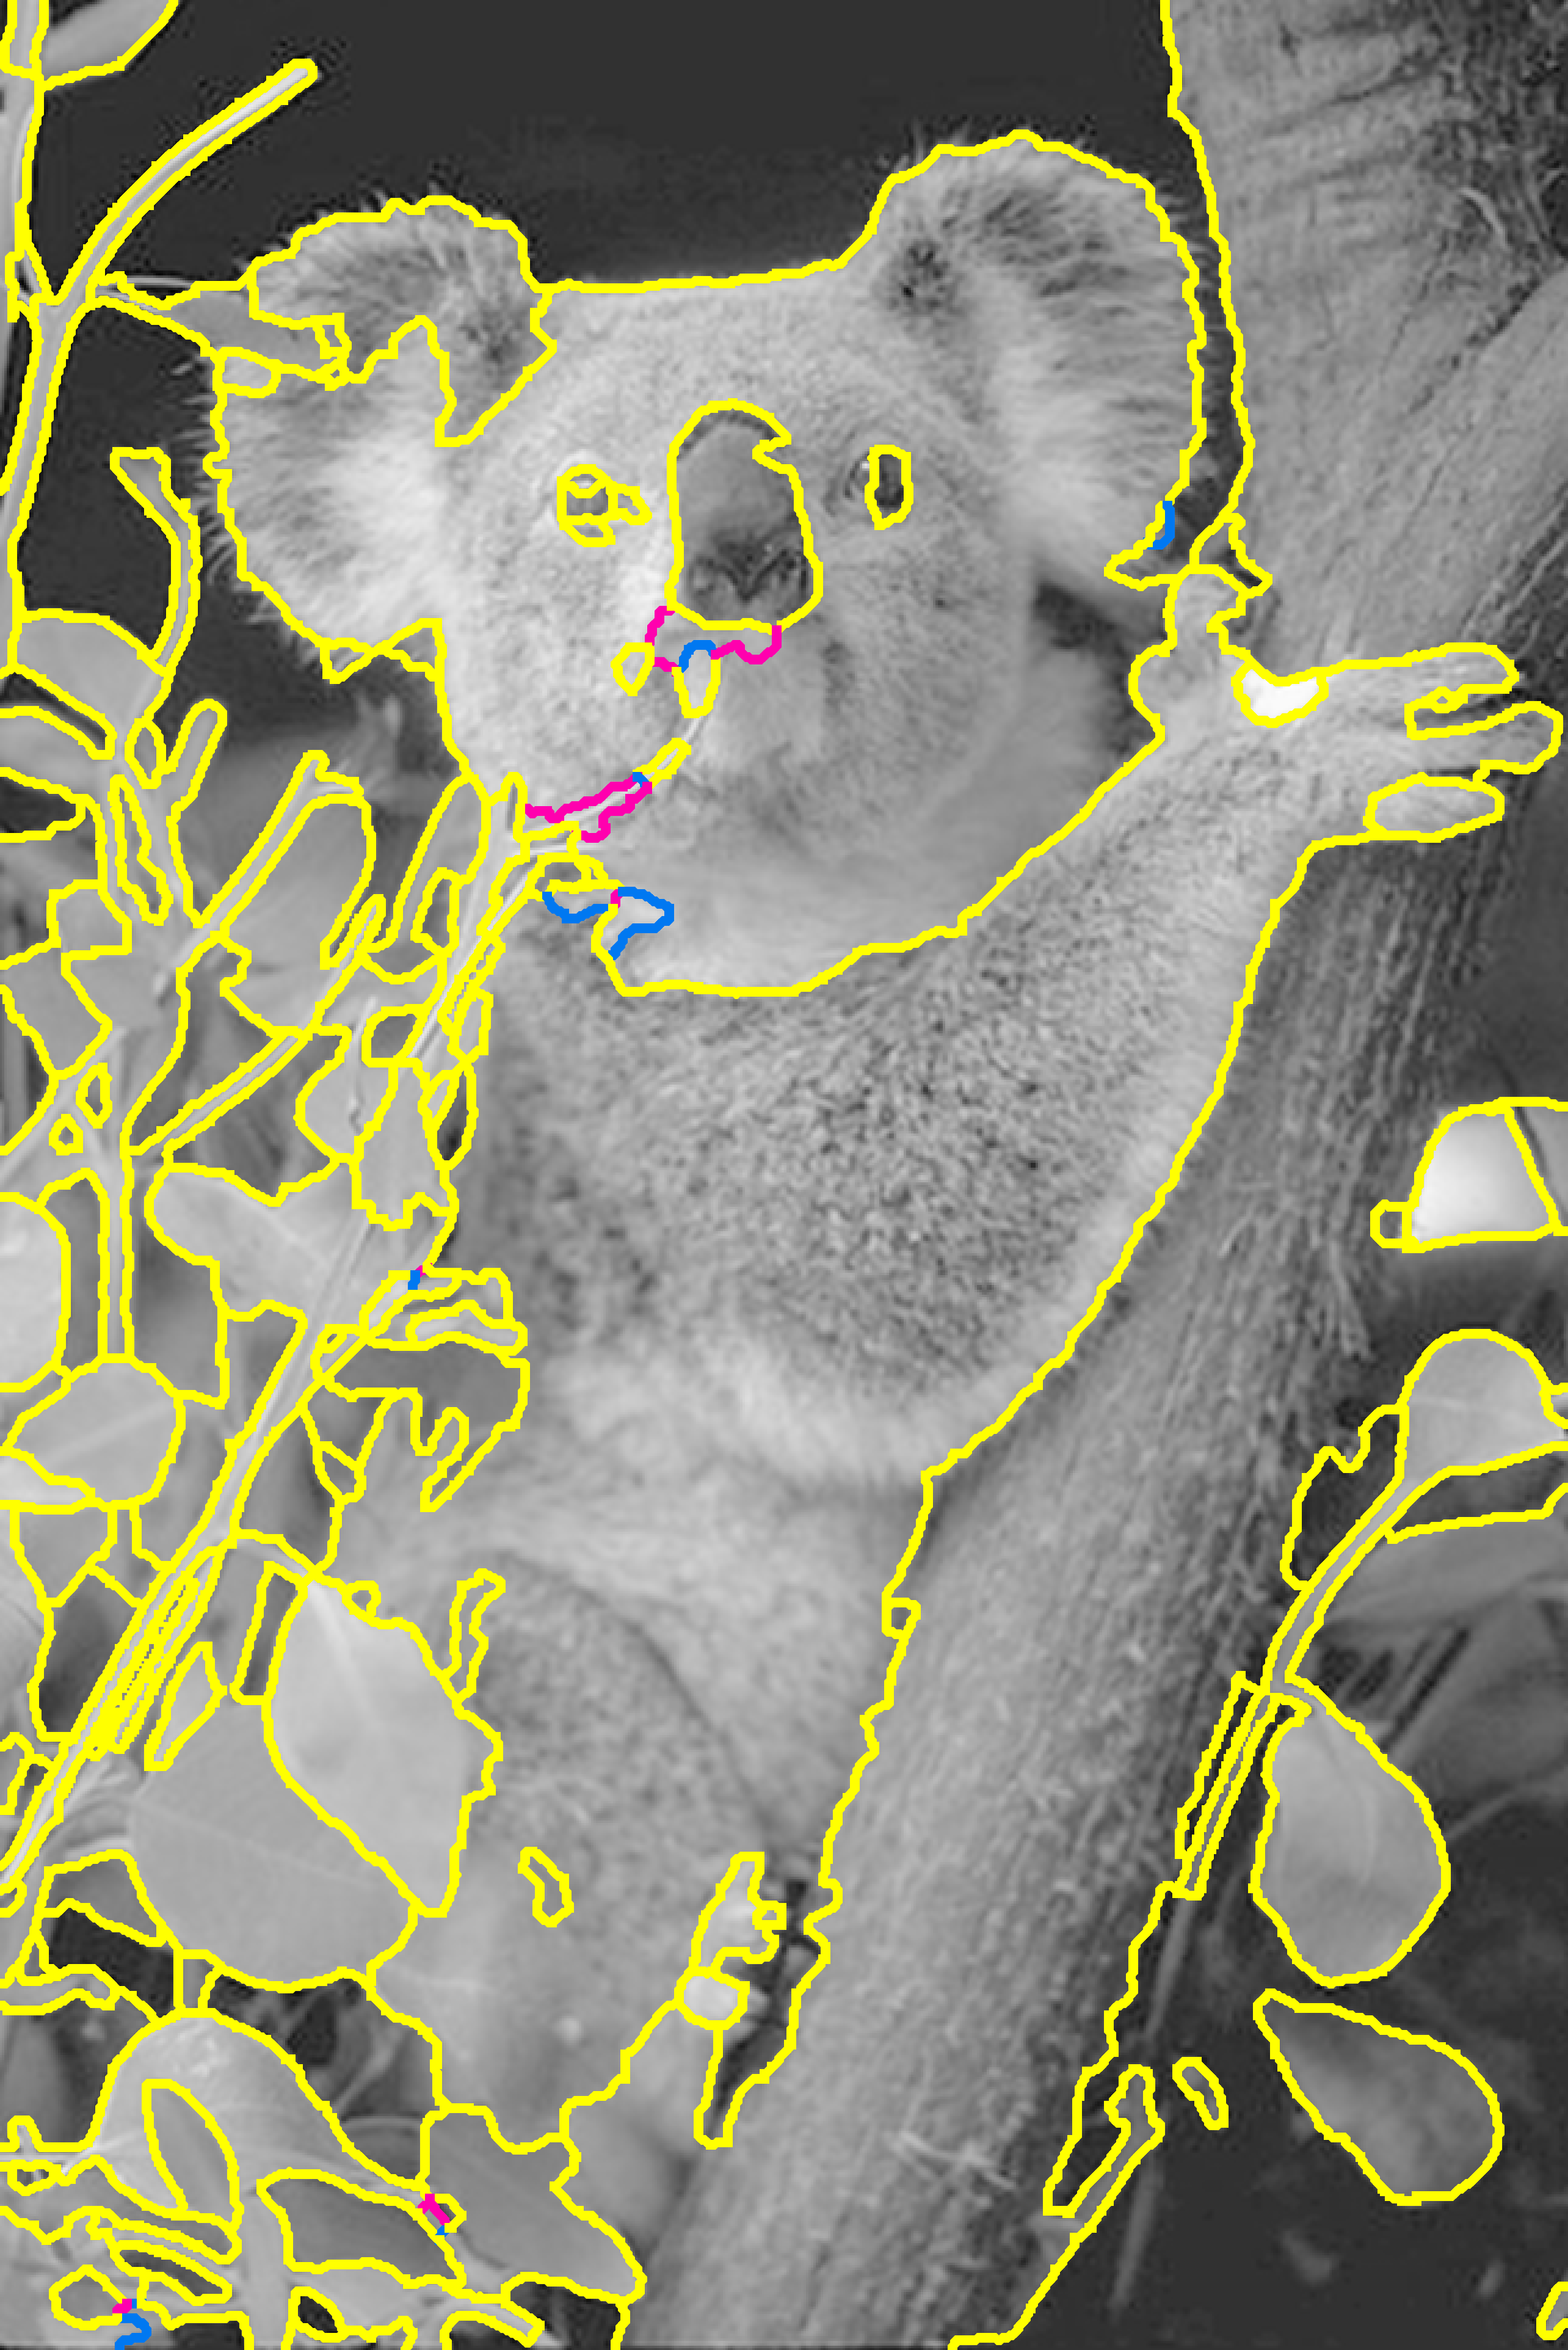
\includegraphics[width=0.17\textwidth]{%
fig/visualcompare/69015_planarcc.png%
}}~%
\subfloat[Expand-and-Explore]{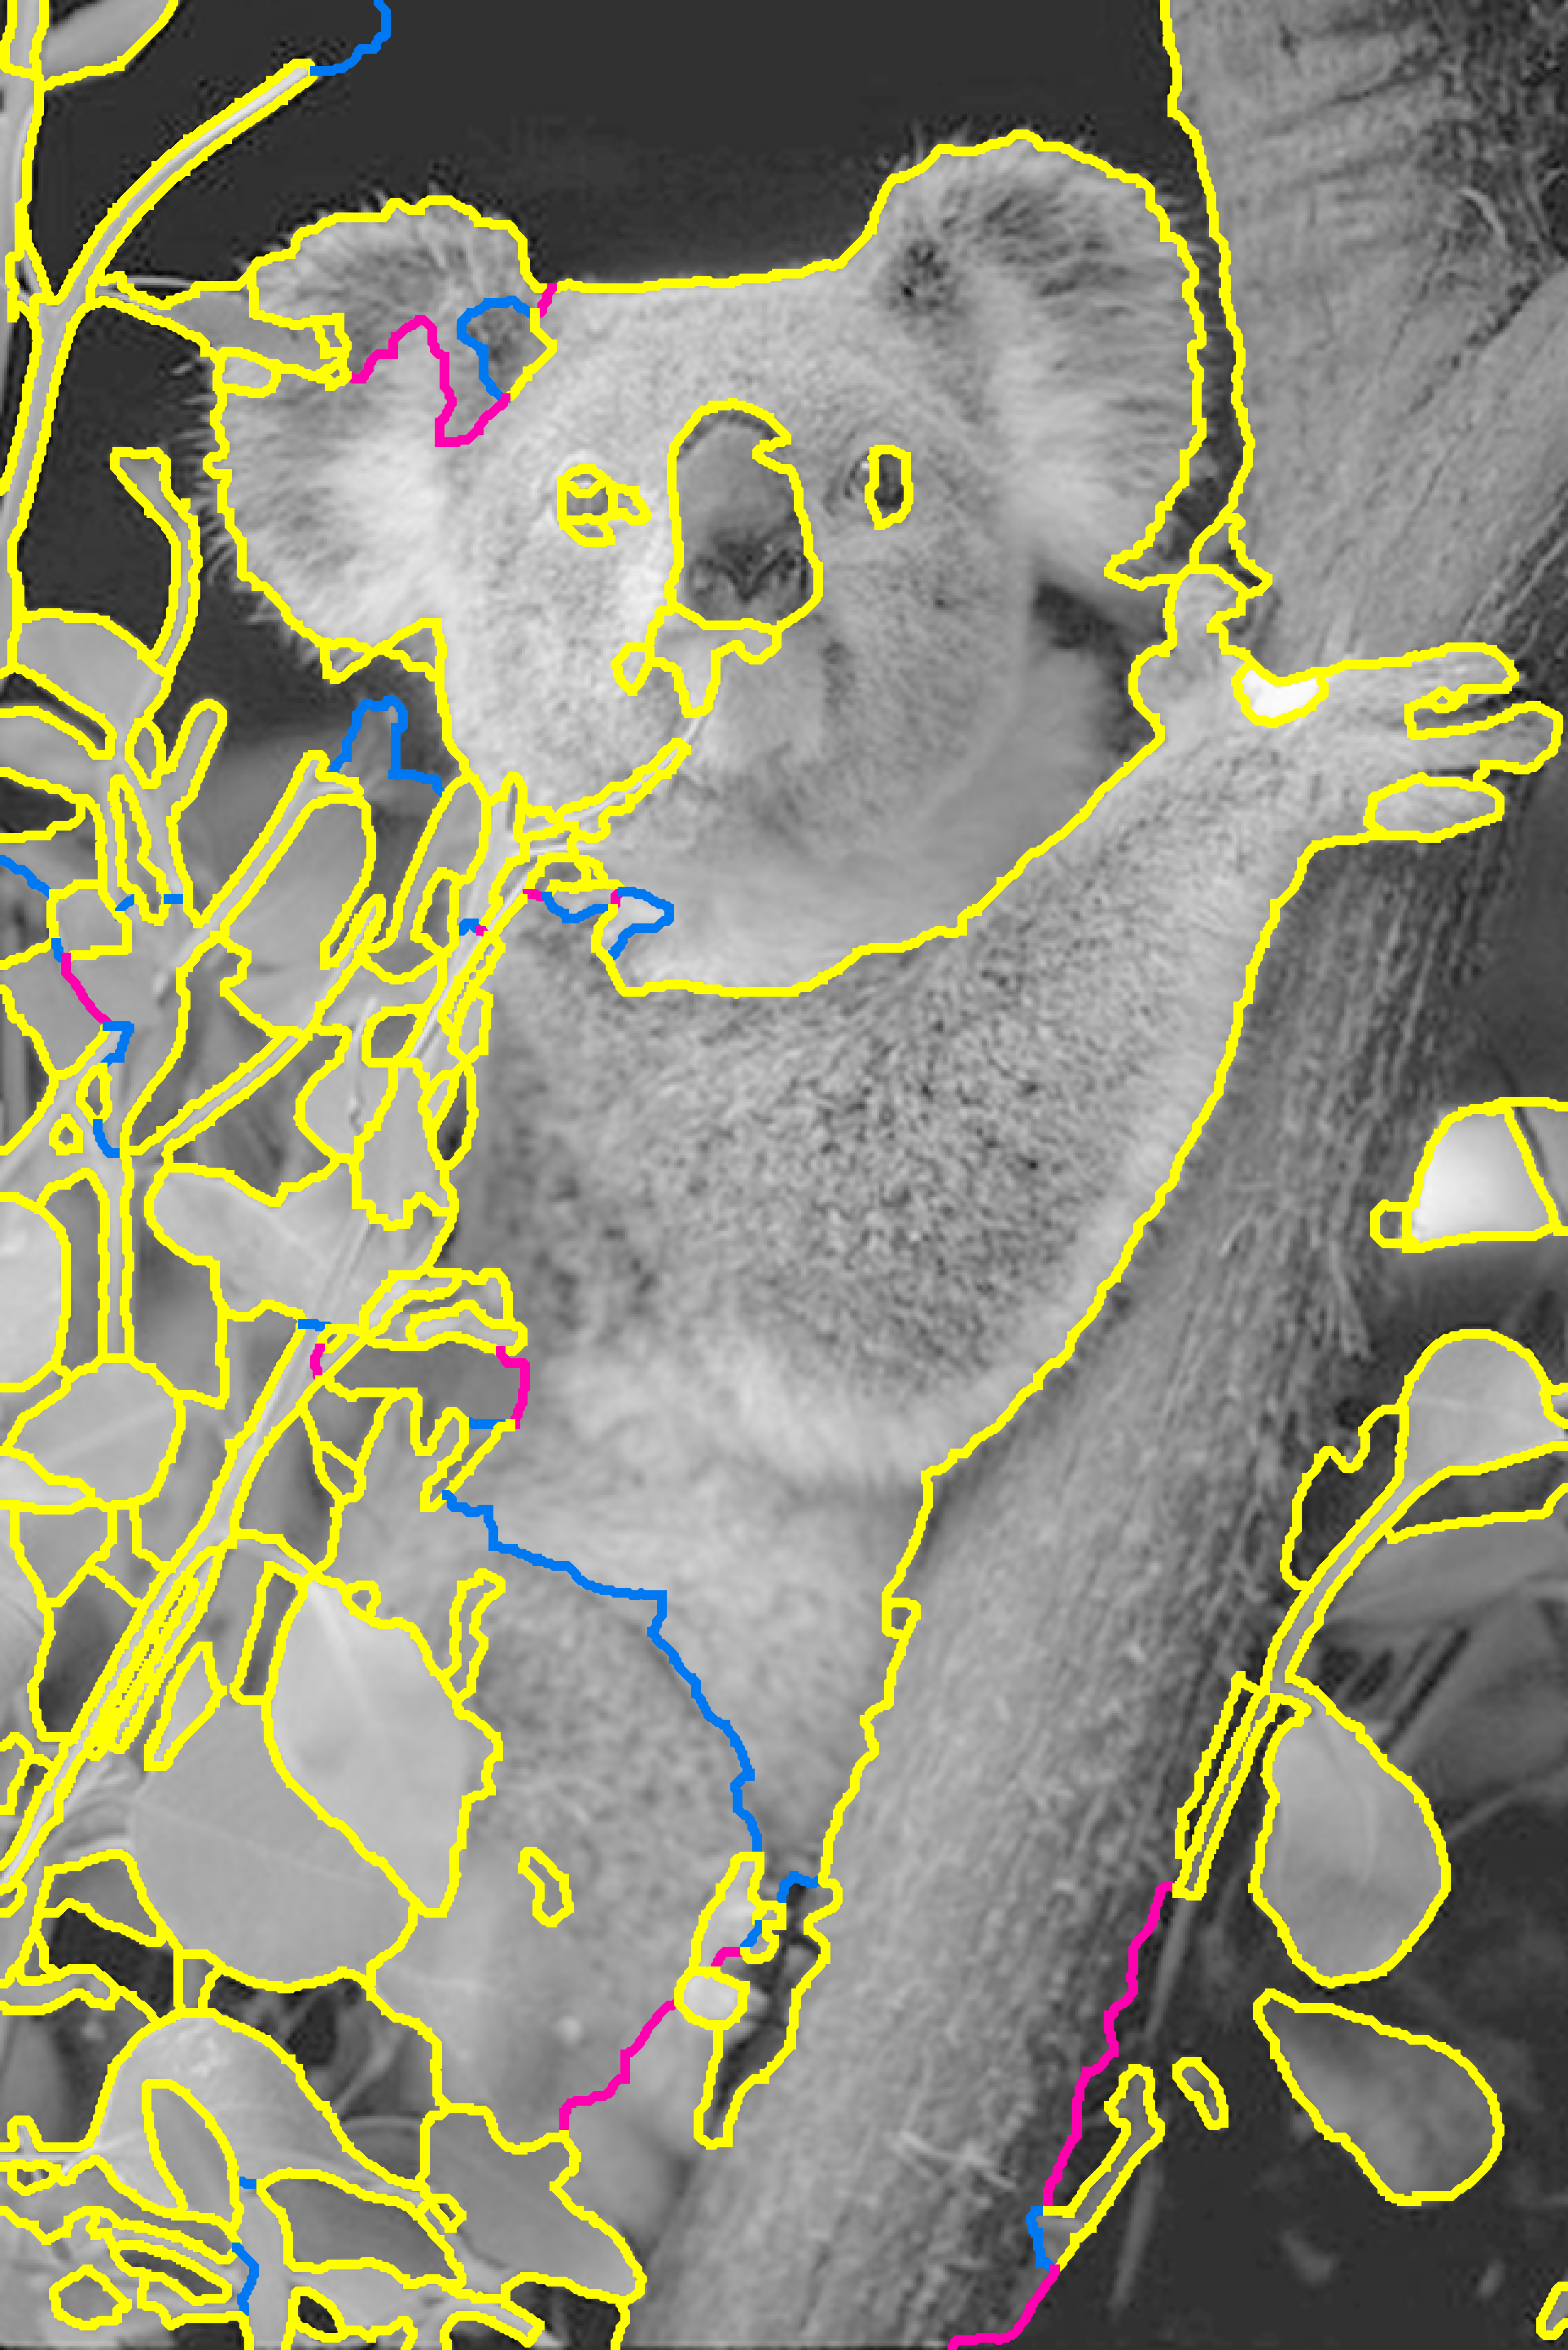
\includegraphics[width=0.17\textwidth]{%
fig/visualcompare/69015_aexpcc.png%
}}~%
\subfloat[Kerninghan-Lin]{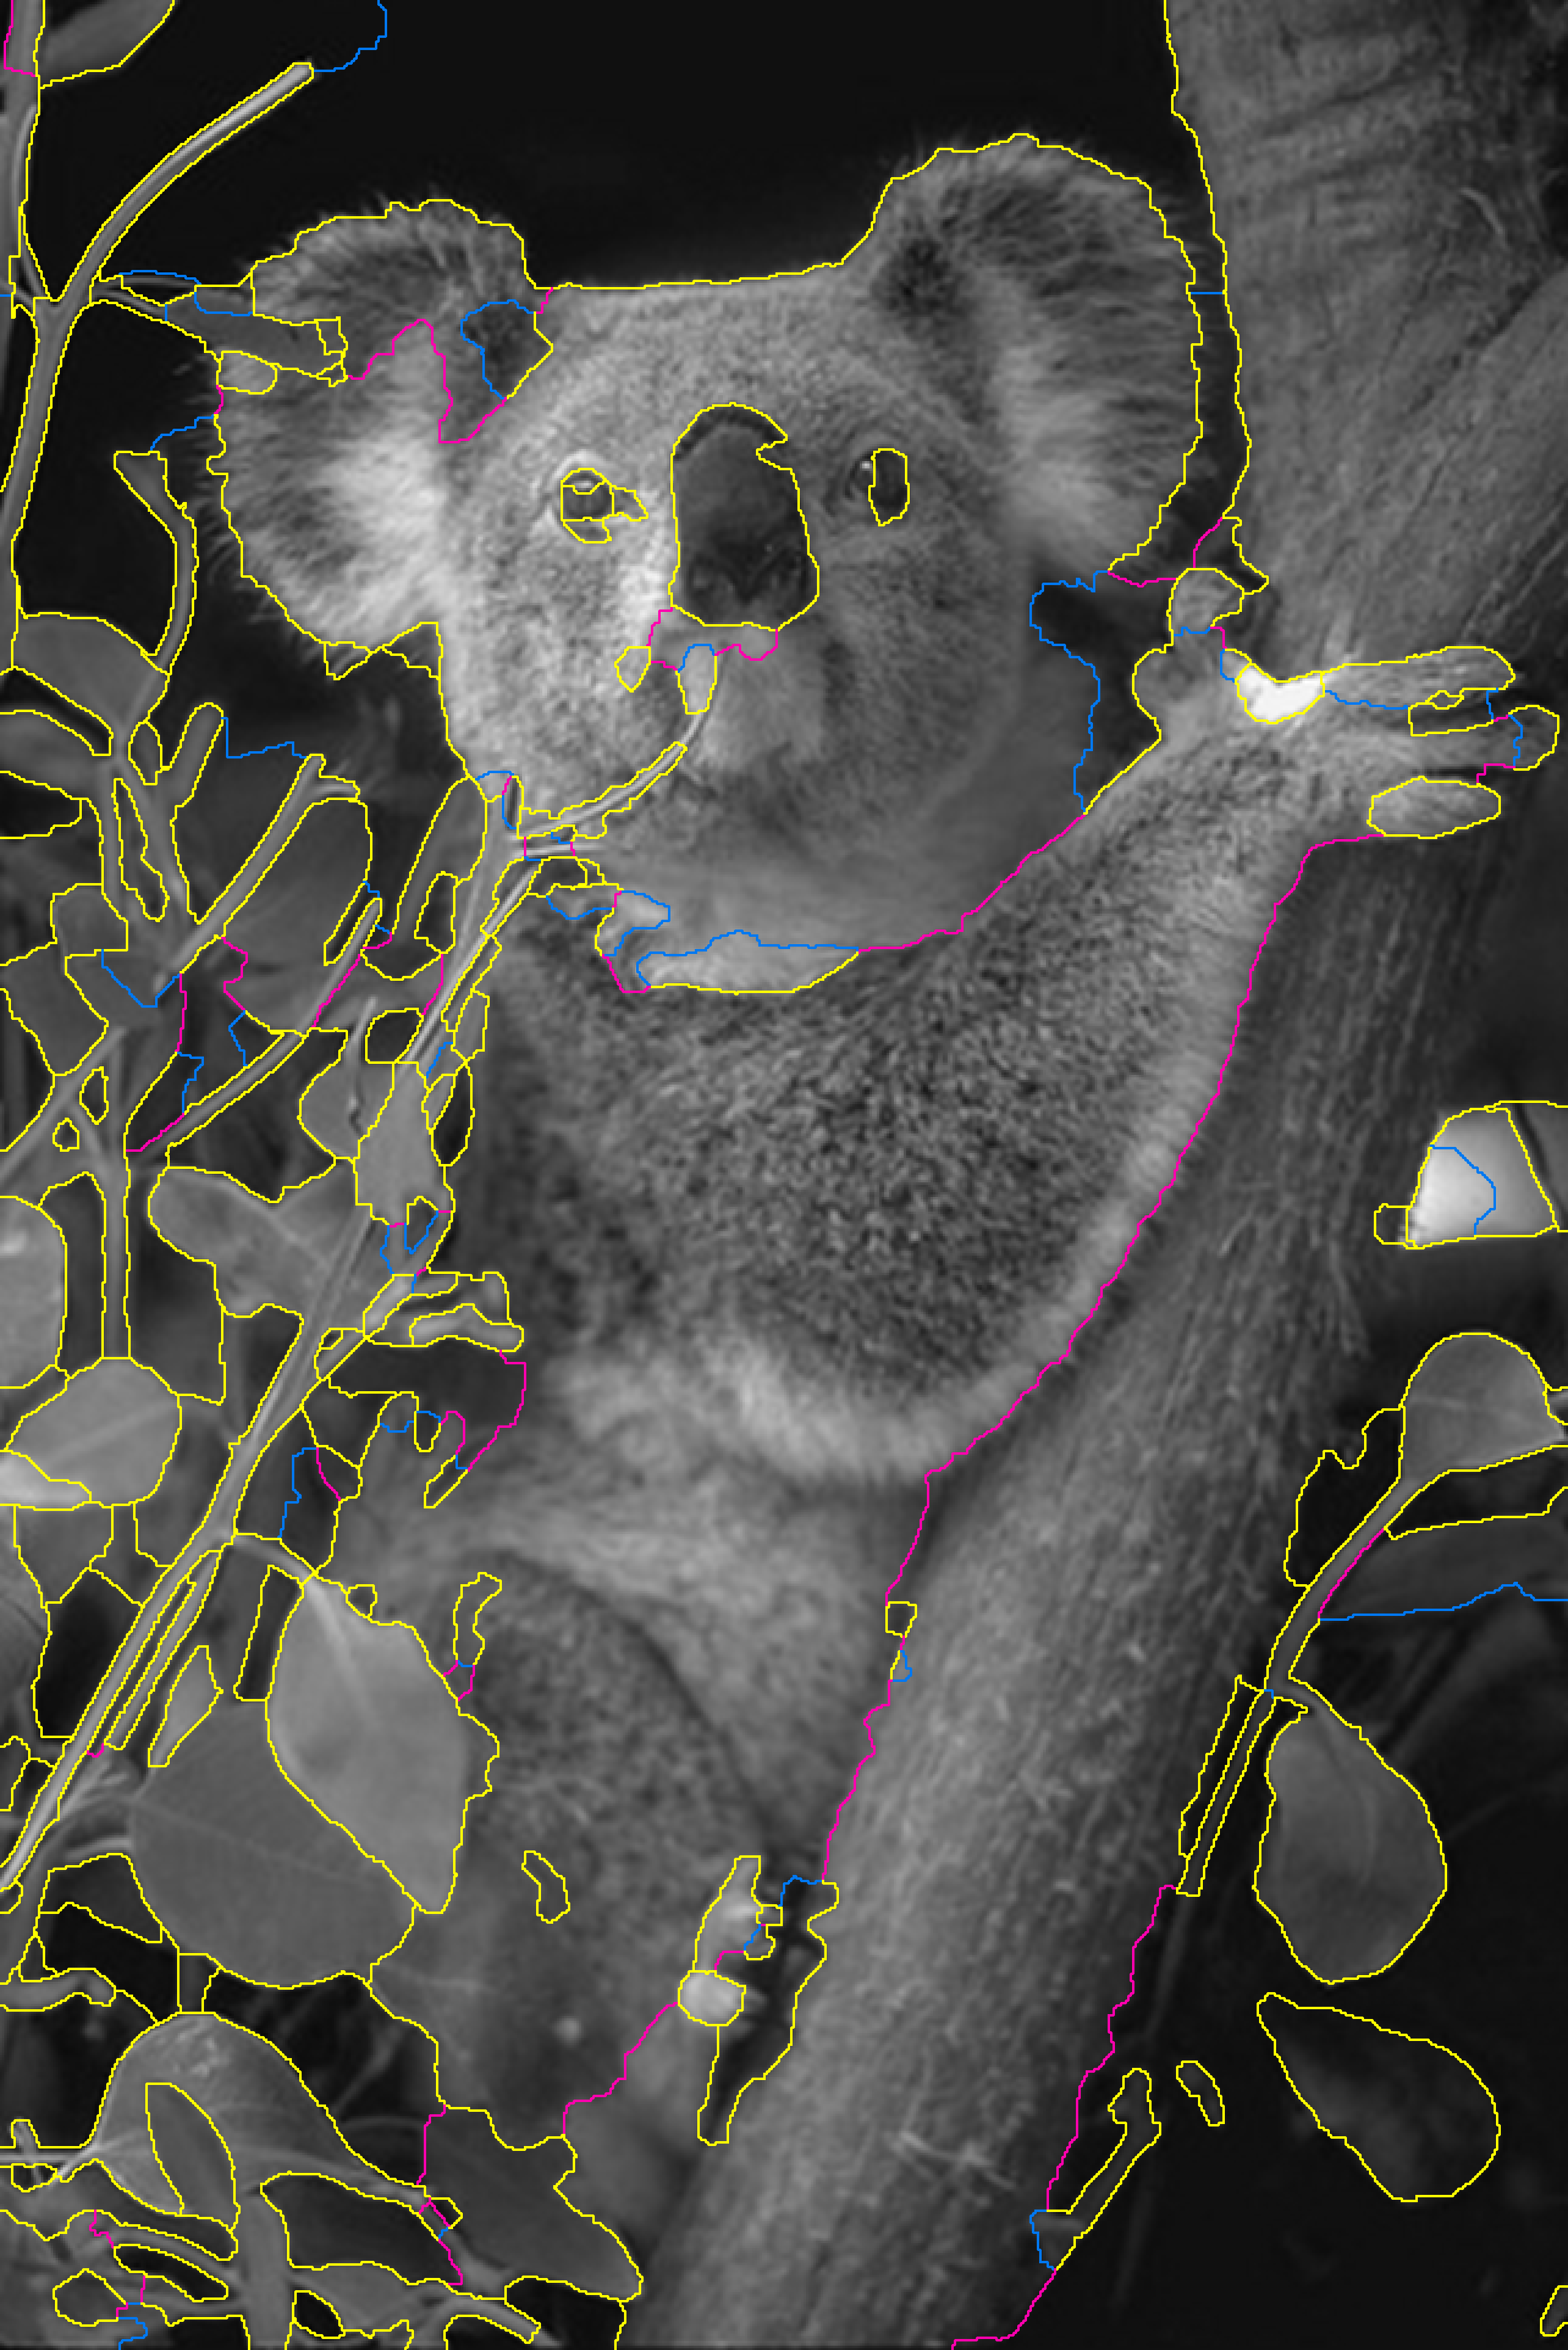
\includegraphics[width=0.17\textwidth]{%
fig/visualcompare/69015_KL.png%
}}
\caption{Comparison of the different multicut algorithms for a model
from \cite{andres_2011_iccv}, based on the superpixel segmentation in (b).
%
The colored boundaries indicate true positives (yellow), false negatives (red),
false positives (blue) and true negatives (invisible) with respect to the
globally optimal solution (f).
\textbf{Top:} %
The image (a) is partitioned into superpixels (b).
A single two-coloring leads to (c) and the cut phase ends with (d).
The final output of the CGC algorithm is (e).
\textbf{Bottom:} %
Results of various competitive methods.
\label{fig:cgc_illustration}}
\end{figure*}
\fi

\section{Experiments\label{sec:experiments}}
We evaluate the performance of our Cut, Glue \& Cut algorithm on
two different 2D segmentation benchmarks as well as
on a new 3D volume segmentation benchmark%
\footnote{Models available at \url{http://on-publication.org}}.

\paragraph{Algorithms.}
For our CGC algorithm, we consider three variants:
CGC-$\ol{B}$ does not do book-keeping, CGC-$\ol{P}$ does not use
the globally optimal Blossom solver for planar max-cut problems,
but rather uses the approximate \mbox{QPBO-I}.
CGC-$\ol{PB}$ does not do book-keeping while using \mbox{QPBO-I} as
max-cut solver.

We compare against the following algorithms:
Kerninghan-Lin (KL, \cite{kerninghan_1970_bell}),
%Iterated Conditional Modes (ICM),
%Lazy Flipper (LF, \cite{andres_2012_eccv_lazy}),
Planar Correlation Clustering (PlanarCC, \cite{yarkony_2012_eccv}),
Expand-and-Explore \cite{bagon_2011_arxiv},
LP-based cutting plane method of a relaxed problem (MC-R),
integer linear program based cutting plane method
(MC-I), which always finds the globally optimal solution.
MC-R and MC-I use facet-defining
separation procedures and bounding techniques as described in
\cite{kappes_2013_arxiv}.
%TODO
%and, as a baseline, Threshold (see below).
%
We use the publicly available C++ implementation in
OpenGM 2.1.1~\cite{andres_2012_opengm_arxiv}
for KL, MC-R and MC-I.
%
For Expand-and-Explore, we use the publicly available code%
\footnote{\url{http://www.wisdom.weizmann.ac.il/~bagon}}
of the corresponding authors. For PlanarCC, we kindly obtained
the implementation by the authors of \cite{yarkony_2012_eccv}.
%
While both are implemented
in MATLAB, all computation-heavy parts are delegated
to C++ functions via MEX wrappers, such that our comparison is fair.

For PlanarCC,
we follow the suggestion of the authors
to stop the algorithm after 40 iterations for better 
runtime. Without this, for several instances,
PlanarCC does not converge after one hour.
With more iterations, the energy of the solutions improves slightly
but at the expense of significantly longer runtime.

Note that in the Expand-and-Explore algorithm,
each binary sub-problem includes by construction unary terms,
%which are generated by fixing one label to alpha
which leads to non-planar sub-problems even when the original
problem is planar.
%Consequently, efficient and exact solving of sub-problems
%is not possible. 

%\emph{Threshold}: this baseline algorithm systematically applies different thresholds
%to the edge weights $\w$, computes the connected components after
%removing edges above the threshold and returns the result which has lowest energy.\\
%%

\paragraph{2D segmentation}
We consider planar 2D segmentation problems derived from the
Berkeley segmentation database: 
\begin{inparaenum}[(i)]
\item
models from \cite{andres_2011_iccv} (BSD300 test data, 100 instances)
and
\item
models from \cite{yarkony_2012_eccv} (BSD300 training data, 200 instances)%
\end{inparaenum}.
%
While the former uses local edge likelihoods learned by a Random forest,
the latter uses global probability of boundary (gPb).
%
Furthermore, they are distinguished in the way they derive the edge weights
$\w$ from the edge probabilities $\vec{p}_e$.
In \cite{andres_2011_iccv},
\begin{equation}
\w_e = \log\left(\frac{\vec{p}(\y_e=0)}{\vec{p}(\y_e=1)}\right)
   + \log\frac{1-\beta}{\beta}
\end{equation}
is chosen while \cite{yarkony_2012_eccv} use
\begin{equation}
\w_e = \log\left(\frac{1-\text{gPb}_e}{\text{gPb}_e}\right)+\gamma.
\end{equation}

Results for both datasets and different values of $\beta$ and $\gamma$
are shown in \cref{fig:experiments-cgc-2d}
%
MC-I finds the global optimum for all instances. The left plots
show the average energy distance (mean gap) to the optimum.
%
Among all approximate methods, CGC performs best.
%
Concerning runtimes, 
CGC has robustly low runtime for a wide range of parameters $\beta, \gamma$.
%

A more detailed comparison for $\beta=0.33$,
as used in \cite{kappes_2013_benchmark_cvpr},
and $\gamma=0.3$ can be found
in \cref{tab:experiments-andres-2d} and \cref{tab:experiments-yarkony-2d-2d}.
These tables additionally show how often the methods find the global
optimum (best), and how often they were able to verify the optimality
by themselves (ver. opt).
%
For \cref{tab:experiments-andres-2d}, groundtruth segmentations
and superpixels were available, such that we can calculate the
Variation of Information (VI, \cite{meila_2003_ltkm}).
%
Interestingly, the globally optimal
solution does not necessarily give the best segmentation as measured by the 
VI (but approximately, VI distance gets larger with
increasing energy as expected).
%
This means that in practice,
it is sufficient to run the much faster CGC
algorithm, see also \cref{fig:cgc_illustration}.

%TODO: cross reference the tables
%Tabs.~\ref{tab:experiments-andres-2d}, \ref{tab:experiments-yarkony-2d} 

%%%%%%%%%%%%%%%%%%%%%%%%%%%%%%%%%%%%%%%%%%%%%%%%%%%%%%%%%%%%%%%%%%%%%%%%%%%%%%%
% fig:experiments-yarkony-2d
%%%%%%%%%%%%%%%%%%%%%%%%%%%%%%%%%%%%%%%%%%%%%%%%%%%%%%%%%%%%%%%%%%%%%%%%%%%%%%%
\begin{center}
\begin{figure*}\label{fig:experiments-cgc-2d}
    \centering
    \subfloat[Evaluation on the planar model from \cite{yarkony_2012_eccv} for different boundary penalties $\gamma$, averaged over 200 instances]
    {
        \label{fig:plots:2d-yarkony-gap}
        \begin{tikzpicture}
            \begin{semilogyaxis}[
                xlabel = {$\gamma$},
                ylabel = {mean gap to optimum},
                xmin = 0,
                xmax = 3,
                ymin = 0,
                ymax = 32,
                mark size=1pt,
                xtick       = {0, 0.5, 1, 1.5, 2, 2.5,3},
                xticklabels = {$0$, $0.5$, $1$, $1.5$, $2$, $2.5$, $3$},
                ytick       = {0.125,0.25,0.5,1, 2,      4,8,16},
                yticklabels = {$0.125$,$0.25$,$0.5$,$1$, $2$,$4$,$8$,$16$},
                width = 0.8\textwidth,
                height=5cm,
                legend style = {draw=none, at={(1.05, 0.5)}, anchor=west, font=\small},
                legend columns = 1
                ]
                \addplot[smooth,mark=\SYMBOLplanarcc,COLOR_planarcc,line width=\thickline] table[x=th, y=PlanarCC]{data/planar-image-seg-V.data};
                \addlegendentry{Planar-CC} 
                \addplot[smooth,mark=\SYMBOLaexpcc,COLOR_aexpcc,line width=\thickline] table[x=th, y=AExpCC]{data/planar-image-seg-V.data};
                \addlegendentry{\ExpAndExplore} 
                \addplot[smooth,mark=\SYMBOLcgc,COLOR_cgc,line width=\thickline] table[x=th, y=CGC]{data/planar-image-seg-V.data};
                \addlegendentry{CGC} 
                \addplot[smooth,mark=\SYMBOLcgcp,yellow,line width=\thickline] table[x=th, y=CGCQPBOI]{data/planar-image-seg-V.data};
                \addlegendentry{CGC-$\ol{P}$} 
                \addplot[smooth,mark=\SYMBOLmcr,COLOR_mcr,line width=\thickline] table[x=th, y=MCR]{data/planar-image-seg-V.data};
                \addlegendentry{MC-R}  
                \addplot[smooth,mark=\SYMBOLmci,COLOR_mci,line width=\thickline] table[x=th, y=MCI]{data/planar-image-seg-V.data};
                \addlegendentry{MC-I} 
                \addplot[smooth,mark=\SYMBOLkl,COLOR_kl,line width=\thickline] table[x=th, y=KL]{data/planar-image-seg-V.data};
                \addlegendentry{KL}  
            \end{semilogyaxis}
        \end{tikzpicture} \newline
    }

    \subfloat[Evaluation on the planar model from \cite{yarkony_2012_eccv} for different boundary penalties $\gamma$, averaged over 200 instances]
    {
        \label{fig:plots:2d-yarkony-time}
        \begin{tikzpicture}
            \begin{semilogyaxis}[
                xlabel = {$\gamma$},
                ylabel = {mean runtime (sec.)},
                xmin = 0,
                xmax = 3,
                ymin = 0,
                ymax = 64,
                mark size=1pt,
                xtick       = {0, 0.5, 1, 1.5, 2, 2.5,3},
                xticklabels = {$0$, $0.5$, $1$, $1.5$, $2$, $2.5$, $3$},
                ytick       = {0.05,0.25, 1,4,8,32},
                yticklabels = {$0.05$,$0.25$,$1$,$4$,$8$,$32$},
                width = 0.8\textwidth,
                height=5cm,
                legend style = {draw=none, at={(1.05, 0.5)}, anchor=west, font=\small},
                legend columns = 1
                ]
                \addplot[smooth,mark=\SYMBOLplanarcc,COLOR_planarcc,line width=\thickline] table[x=th, y=PlanarCC]{data/planar-image-seg-T.data};
                \addlegendentry{Planar-CC} 
                \addplot[smooth,mark=\SYMBOLaexpcc,COLOR_aexpcc, line width=\thickline] table[x=th, y=AExpCC]{data/planar-image-seg-T.data};
                \addlegendentry{\ExpAndExplore} 
                \addplot[smooth,mark=\SYMBOLcgc,COLOR_cgc, line width=\thickline] table[x=th, y=CGC]{data/planar-image-seg-T.data};
                \addlegendentry{CGC} 
                \addplot[smooth,mark=\SYMBOLcgcp,COLOR_cgcp, line width=\thickline] table[x=th, y=CGCQPBOI]{data/planar-image-seg-T.data};
                \addlegendentry{CGC-$\ol{P}$} 
                \addplot[smooth,mark=\SYMBOLmcr,COLOR_mcr, line width=\thickline] table[x=th, y=MCR]{data/planar-image-seg-T.data};
                \addlegendentry{MC-R}  
                \addplot[smooth,mark=\SYMBOLmci,COLOR_mci, line width=\thickline] table[x=th, y=MCI]{data/planar-image-seg-T.data};
                \addlegendentry{MC-I} 
                \addplot[smooth,mark=\SYMBOLkl,COLOR_kl, line width=\thickline] table[x=th, y=KL]{data/planar-image-seg-T.data};
                \addlegendentry{KL}  
                %\addplot[dashed,COLOR_planarcc] table[x=th, y=MedPlanarCC]{data/planar-image-seg-T.data};
                %\addplot[dashed,COLOR_aexpcc  ] table[x=th, y=MedAExpCC  ]{data/planar-image-seg-T.data};
                %\addplot[dashed,COLOR_cgc     ] table[x=th, y=MedCGC     ]{data/planar-image-seg-T.data};
                %\addplot[dashed,COLOR_cgcp    ] table[x=th, y=MedCGCQPBOI]{data/planar-image-seg-T.data};
                %\addplot[dashed,COLOR_mcr     ] table[x=th, y=MedMCR     ]{data/planar-image-seg-T.data};
                %\addplot[dashed,COLOR_mci     ] table[x=th, y=MedMCI     ]{data/planar-image-seg-T.data};
                %\addplot[dashed,COLOR_kl      ] table[x=th, y=MedKL      ]{data/planar-image-seg-T.data};
            \end{semilogyaxis}
        \end{tikzpicture}
        \vspace*{-0.3cm}  
    }

    \subfloat[Evaluation on the planar models from~\cite{andres_2011_iccv} for different boundary penalties $(\beta)$, averaged over 100 instances]
    {
        \label{fig:plots:2d-andres-gap}
        \begin{tikzpicture}
            \begin{semilogyaxis}[
                xlabel = {\footnotesize{$\beta$}},
                ylabel = {mean gap to optimum},
                xmin = 0,
                xmax = 1,
                ymin = 0,
                ymax = 64,
                mark size=1pt, 
                xtick       = {0.1, 0.5, 0.9},
                xticklabels = {$0.1$, $0.5$, $0.9$},
                ytick       = {0.125,0.25,0.5,1, 2,      4,8,16,32,64},
                yticklabels = {$0.125$,$0.25$,$0.5$,$1$, $2$,$4$,$8$,$16$,$32$,$64$},
                width = 0.8\textwidth,
                height=5cm,
                legend style = {draw=none, at={(1.05, 0.5)}, anchor=west, font=\small},
                legend columns = 1
                ]
                \addplot[smooth,mark=\SYMBOLplanarcc,COLOR_planarcc,line width=\thickline] table[x=th, y=PlanarCC]{data/image-seg-b-V.data};
                \addlegendentry{Planar-CC} 
                \addplot[smooth,mark=\SYMBOLaexpcc,COLOR_aexpcc,line width=\thickline] table[x=th, y=AExpCC]{data/image-seg-b-V.data};
                \addlegendentry{\ExpAndExplore} 
                \addplot[smooth,mark=\SYMBOLcgc,COLOR_cgc,line width=\thickline] table[x=th, y=CGC]{data/image-seg-b-V.data};
                \addlegendentry{CGC} 
                \addplot[smooth,mark=\SYMBOLcgcp,COLOR_cgcp,line width=\thickline] table[x=th, y=CGCQPBOI]{data/image-seg-b-V.data};
                \addlegendentry{CGC-$\ol{P}$} 
                \addplot[smooth,mark=\SYMBOLmcr,COLOR_mcr,line width=\thickline] table[x=th, y=MCR]{data/image-seg-b-V.data};
                \addlegendentry{MC-R}  
                \addplot[smooth,mark=\SYMBOLmci,COLOR_mci,line width=\thickline] table[x=th, y=MCI]{data/image-seg-b-V.data};
                \addlegendentry{MC-I} 
                \addplot[smooth,mark=\SYMBOLkl,COLOR_kl,line width=\thickline] table[x=th, y=KL]{data/image-seg-b-V.data};
                \addlegendentry{KL} 
            \end{semilogyaxis}
        \end{tikzpicture} 
    }

    \subfloat[Evaluation on the planar models from~\cite{andres_2011_iccv} for different boundary penalties $(\beta)$, averaged over 100 instances]
    {
        \label{fig:plots:2d-andres-time}
        \begin{tikzpicture}
            \begin{semilogyaxis}[
                xlabel = {\footnotesize{$\beta$}},
                ylabel = {mean runtime (sec.)},
                xmin = 0,
                xmax = 1,
                ymin = 0,
                ymax = 64,
                mark size=1pt,
                xtick       = {0.1, 0.5, 0.9},
                xticklabels = {$0.1$, $0.5$, $0.9$},
                ytick       = {0.05,0.25, 1,4,8,32},
                yticklabels = {$0.05$,$0.25$,$1$,$4$,$8$,$32$},
                width = 0.8\textwidth,
                height=5cm,
                legend style = {draw=none, at={(1.05, 0.5)}, anchor=west, font=\small},
                legend columns = 1
                ]
                \addplot[smooth,mark=\SYMBOLplanarcc,COLOR_planarcc,line width=\thickline] table[x=th, y=PlanarCC]{data/image-seg-b-T.data};
                \addlegendentry{Planar-CC} 
                \addplot[smooth,mark=\SYMBOLaexpcc,COLOR_aexpcc,line width=\thickline] table[x=th, y=AExpCC]{data/image-seg-b-T.data};
                \addlegendentry{\ExpAndExplore} 
                \addplot[smooth,mark=\SYMBOLcgc,COLOR_cgc,line width=\thickline] table[x=th, y=CGC]{data/image-seg-b-T.data};
                \addlegendentry{CGC} 
                \addplot[smooth,mark=\SYMBOLcgcp,COLOR_cgcp,line width=\thickline] table[x=th, y=CGCQPBOI]{data/image-seg-b-T.data};
                \addlegendentry{CGC-$\ol{P}$} 
                \addplot[smooth,mark=\SYMBOLmcr,COLOR_mcr,line width=\thickline] table[x=th, y=MCR]{data/image-seg-b-T.data};
                \addlegendentry{MC-R}  
                \addplot[smooth,mark=\SYMBOLmci,COLOR_mci,line width=\thickline] table[x=th, y=MCI]{data/image-seg-b-T.data};
                \addlegendentry{MC-I} 
                \addplot[smooth,mark=\SYMBOLkl,COLOR_kl,line width=\thickline] table[x=th, y=KL]{data/image-seg-b-T.data};
                \addlegendentry{KL} 
                %\addplot[dashed,COLOR_planarcc] table[x=th, y=MedPlanarCC]{data/image-seg-b-T.data};
                %\addplot[dashed,COLOR_aexpcc  ] table[x=th, y=MedAExpCC  ]{data/image-seg-b-T.data};
                %\addplot[dashed,COLOR_cgc     ] table[x=th, y=MedCGC     ]{data/image-seg-b-T.data};
                %\addplot[dashed,COLOR_cgcp    ] table[x=th, y=MedCGCQPBOI]{data/image-seg-b-T.data};
                %\addplot[dashed,COLOR_mcr     ] table[x=th, y=MedMCR     ]{data/image-seg-b-T.data};
                %\addplot[dashed,COLOR_mci     ] table[x=th, y=MedMCI     ]{data/image-seg-b-T.data};
                %\addplot[dashed,COLOR_kl      ] table[x=th, y=MedKL      ]{data/image-seg-b-T.data};
            \end{semilogyaxis}
        \end{tikzpicture}
    }

    \caption{%
Evaluation on various benchmark datasets:
\Cref{fig:plots:2d-yarkony-gap} and \cref{fig:plots:2d-andres-gap} :
Gap to the global optimal energy (MC-I) averaged over all instances.
\Cref{fig:plots:2d-yarkony-time} and \cref{fig:plots:2d-andres-time} :
Mean runtime of the methods.
For both 2D images,
CGC outperforms all competitors in terms of runtime and CGC gives better results in
terms of energy than all competitive approximative methods.
Only Integer Multicut (MC-I) gives better partitions in terms of energy but is
significantly slower.
}

\end{figure*}
\end{center}




\begin{center}
\begin{figure*}\label{fig:experiments-cgc-3d}

    \subfloat[Evaluation on a new 3D segmentation benchmark for different volume sizes $N^3$ averaged over 8 instances]
    {%
        \label{fig:plots:3d:gap}
        \begin{tikzpicture}
            \begin{axis}[
                xlabel = {\footnotesize{$N$}},
                ylabel = {distance to optimal energy},
                xmin = 0,
                xmax = 550,
                ymin = 0,
                ymax = 1000,
                mark size=1pt,
                xtick       = {90, 150, 300, 450, 550},
                xticklabels = {$90$, $150$, $300$, $450$, $550$}, 
                %=ytick       = {0,-1000, -10000,-100000},
                %yticklabels = {$0$,$-10^3$,$-10^4$,$-10^5$},
                width = 0.8\textwidth,
                height=5cm,
                legend style = {draw=none, at={(1.05, 0.5)}, anchor=west, font=\small},
                legend columns = 1
                ]
                \addplot[mark=\SYMBOLaexpcc,COLOR_aexpcc, line width=\thickline] table[x=N, y=AExpCC]{data/knott-V2.data};
                \addlegendentry{Expand \& Explore} 
                \addplot[mark=\SYMBOLcgcp,COLOR_cgcp, line width=\thickline] table[x=N, y=CGCQPBOI]{data/knott-V2.data}; 
                \addlegendentry{CGC$-{\ol{P}}$}
                \addplot[mark=\SYMBOLmcr,COLOR_mcr, line width=\thickline] table[x=N, y=MCR]{data/knott-V2.data};
                \addlegendentry{MC-R} 
                \addplot[mark=\SYMBOLmci,COLOR_mci, line width=\thickline] table[x=N, y=MCI]{data/knott-V2.data};
                \addlegendentry{MC-I} 
                \addplot[mark=\SYMBOLkl,COLOR_kl, line width=\thickline] table[x=N, y=KL]{data/knott-V2.data};
                \addlegendentry{KL}
            \end{axis}
        \end{tikzpicture} 
    }

    \subfloat[Evaluation on a new 3D segmentation benchmark for different volume sizes $N^3$ averaged over 8 instances]
    {%
        \label{fig:plots:3d:time}
        \begin{tikzpicture}
            %\begin{semilogyaxis}[ 
            \begin{axis}[
                xlabel = {\footnotesize{$N$}},
                ylabel = {mean runtime (sec.)},
                xmin = 0,
                xmax = 550,
                ymin = 0,
                ymax = 1200,
                mark size=1pt,
                xtick       = {90, 150, 300, 450, 550},
                xticklabels = {$90$, $150$, $300$, $450$, $550$},
                ytick       = {0, 600,1200},
                yticklabels = {$0$,$600$,$1200$},
                width = 0.8\textwidth,
                height=5cm,
                legend style = {draw=none, at={(1.05, 0.5)}, anchor=west, font=\small},
                legend columns = 1
                ]
                \addplot[smooth,mark=\SYMBOLaexpcc,COLOR_aexpcc,line width=\thickline] table[x=N, y=AExpCC]{data/knott-T2.data};
                \addlegendentry{Expand \& Explore} 
                \addplot[smooth,mark=\SYMBOLcgcp,COLOR_cgcp,line width=\thickline] table[x=N, y=CGCQPBOI]{data/knott-T2.data};
                \addlegendentry{CGC$-{\ol{P}}$}
                \addplot[smooth,mark=\SYMBOLmcr,COLOR_mcr,line width=\thickline] table[x=N, y=MCR]{data/knott-T2.data};
                \addlegendentry{MC-R}  
                \addplot[smooth,mark=\SYMBOLmci,COLOR_mci,line width=\thickline] table[x=N, y=MCI]{data/knott-T2.data};
                \addlegendentry{MC-I} 
                \addplot[smooth,mark=\SYMBOLkl,COLOR_kl,line width=\thickline] table[x=N, y=KL]{data/knott-T2.data};
                \addlegendentry{KL} 
                %\end{semilogyaxis}
            \end{axis}
        \end{tikzpicture}
    }
    \caption{%
    Evaluation on various benchmark datasets.
    \Cref{fig:plots:3d:gap} : Gap to the global optimal energy (MC-I) averaged over all instances.
    \Cref{fig:plots:3d:gap} Mean runtime of the methods.
    For 3D images,
    CGC outperforms all competitors in terms of runtime.
    For 3D volume image segmentation,
    the approximate MC-R method beats CGC, though at significant 
    runtime cost.
    }
\end{figure*}
\end{center}




\begin{table*}
\scriptsize
\centering
\label{tab:experiments-andres-2d}
\begin{tabular}{lrrrrrr}
\toprule
           algorithm &         runtime       &           value &           bound &       best &   ver. opt&              VI  \\\midrule % &     RI \\ \midrule 
                  KL & $         4.96$ sec & $      4608.57$ & $      -\infty$ & $       0$ & $       0$  & $       2.6431$  \\ % & $       0.6401$ \\   
        Expand \& Explore & $         2.90$ sec & $      4486.57$ & $      -\infty$ & $       1$ & $       0$  & $       2.9153$  \\ % & $       0.6527$ \\ 
     %         CGCold & $    {\bf0.42}$ sec & $      4445.10$ & $      4136.83$ & $      23$ & $       0$  & $  {\bf2.5345}$  \\ % & $       0.7780$ \\ 
       CGC-${\ol{PB}}$ & $       6.35$ sec & $      4466.80$ & $      -\infty$ & $       1$ & $       0$  & $   {\bf2.5247}$   \\ %& $       0.7590$ \\ 
        CGC-${\ol{P}}$ & $       5.35$ sec & $      4466.80$ & $      -\infty$ & $       1$ & $       0$  & $   {\bf2.5247}$   \\ %& $       0.7590$ \\ 
        CGC-${\ol{B}}$ & $       0.63$ sec & $      4445.06$ & $      -\infty$ & $      23$ & $       0$  & $       2.5355$   \\ %& $       0.7779$ \\ 
                 CGC & $    {\bf0.42}$ sec & $      4445.06$ & $      -\infty$ & $      23$ & $       0$  & $       2.5355$   \\ %& $       0.7779$ \\ 
\cmidrule{1-1}                                                                                                             
                MC-R & $         5.16$ sec & $      4447.47$ & $      4442.34$ & $      35$ & $      35$  & $       2.5490$  \\ % & $       0.7822$ \\
           Planar-CC & $         5.20$ sec & $      4450.73$ & $      4437.29$ & $       9$ & $       8$  & $       2.5603$  \\ % & $       0.7843$ \\         
\cmidrule{1-1}                                                                                                             
                MC-I & $         2.20$ sec & $ {\bf4442.64}$ & $ {\bf4442.64}$ & ${\bf100}$ & ${\bf100}$  & $       2.5363$  \\ % & $       0.7821$ \\    
\bottomrule                                                               
\end{tabular}\hspace*{1cm}%
\caption{
Summary over the models from \cite{andres_2011_iccv}, 100 instances.
Mean runtime, energy and bound (if available) for different multicut solvers.
Also shown is how often each method finds the global optimum (``best''),
and how often a method is able to verify the optimality by itself
(``ver. opt'').
Execution was aborted after one hour.
Best values are marked in bold.
The VI columns reports the Variation of Information \cite{meila_2003_ltkm}.
}
\end{table*}


\begin{table*}
\centering
\scriptsize
\label{tab:experiments-yarkony-2d-2d}
\begin{tabular}{lrrrrr}
\toprule
           algorithm &         runtime       &           value &           bound &       best &   ver. opt   \\ \midrule 
                  KL & $         0.04$ sec & $       -73.41$ & $      -\infty$ & $      45$ & $       0$ \\
    Expand \& Explore & $    {\bf0.03}$ sec & $       -89.90$ & $      -\infty$ & $     130$ & $       0$ \\ 
       CGC-${\ol{PB}}$ & $   {\bf0.03}$ sec & $       -89.45$ & $      -\infty$ & $     104$ & $       0$ \\ 
        CGC-${\ol{P}}$ & $   {\bf0.03}$ sec & $       -89.45$ & $      -\infty$ & $     104$ & $      0$ \\ 
        CGC-${\ol{B}}$ & $   {\bf0.03}$ sec & $       -92.25$ & $      -\infty$ & $     185$ & $       0$ \\ 
       CGC           & $     {\bf0.03}$ sec & $       -92.25$ & $      -\infty$ & $     185$ & $       0$ \\ 
\cmidrule{1-1} 
                MC-R & $         3.48$ sec & $       -91.70$ & $       -92.39$ & $     181$ & $     180$ \\
           Planar-CC & $         0.36$ sec & $       -92.16$ & $       -92.39$ & $     184$ & $     174$ \\  
\cmidrule{1-1} 
                MC-I & $        29.80$ sec & $       {\bf-92.35}$ & $       \bf{-92.35}$ & $     {\bf200}$ & $     {\bf200}$ \\ 

\bottomrule
\end{tabular}
\caption{
Summary over the models from \cite{yarkony_2012_eccv},
200 instances. 
Mean runtime, energy and bound (if available) for different multicut solvers.
Also shown is how often each method finds the global optimum (``best''),
and how often a method is able to verify the optimality by itself
(``ver. opt'').
Execution was aborted after one hour.
Best values are marked in bold.
Without superpixel maps available, VI could not be
calculated.
}
\end{table*}

%%%%%%%%%%%%%%%%%%%%%%%%%%%%%%%%%%%%%%%%%%%%%%%%%%%%%%%%%%%%%%%%%%%%%%%%%%%%%%%

\paragraph{3D segmentation}
For 3D segmentation, recently Kappes et al.
\cite{kappes_2013_benchmark_cvpr} released a benchmark dataset. However,
this only includes one small and one huge instance. Therefore
the authors of \cite{kroeger_2012_eccv} kindly provided us
with a more comprehensive set of instances
over a range of different problem sizes from volumes of $30^3$ up to 
$450^3$ voxels.
%
Results are shown
in Fig.~\ref{fig:plots:3d}
and for volumes of $400^3$ are detailed in 
Tab.~\ref{tab:smalltable-knott-3d-400}.

Based on the energy difference of CGC and CGC-$\ol{P}$ for the planar models,
we expect reduced performance for the non-planar case of 3D volume image
segmentation (Fig.~\ref{fig:plots:3d}). Still, with a runtime
as fast as KL (the fastest algorithm considered),
CGC-$\ol{P}$ is able to obtain much lower-energy solutions and
lies between MC-I, MC-R and Expand \& Explore.
%
For instances with $400^3$ voxels, MC-I was only able to find for 7 out of 
8 instances the global optimum within one hour
(Tab.~\ref{tab:smalltable-knott-3d-400}).

%%%%%%%%%%%%%%%%%%%%%%%%%%%%%%%%%%%%%%%%%%%%%%%%%%%%%%%%%%%%%%%%%%%%%%%%%%%%%%
% tab:experiments-knott-3d
%%%%%%%%%%%%%%%%%%%%%%%%%%%%%%%%%%%%%%%%%%%%%%%%%%%%%%%%%%%%%%%%%%%%%%%%%%%%%%%
% \begin{table}[H]
% \scriptsize
% \centering
% \caption{knott-3d-400 (8 instances)}
% \label{tab:experiment-knott-3d}
% \begin{tabular}{lrrrrr}
% \toprule
%            algorithm &         runtime       &           value &           bound &       best &   ver. opt   \\ \midrule 
%               ogm-KL & $        85.06$ $(84.51)$ sec & $    -53476.75$ & $      -\infty$ & $       0$ & $       0$ \\ 
% \cmidrule{1-1} 
%         ogm-MC-CCFDB & $      4121.08$ $(4087.66)$ sec & $    -20111.68$ & $    -58774.97$ & $       0$ & $       0$ \\ 
% \cmidrule{1-1} 
%         ogm-MC-CCIFD & $       745.53$ $(286.18)$ sec & $    -57319.41$ & $    -57386.73$ & $       7$ & $       7$ \\ 
% \cmidrule{1-1} 
%           CGC-QPBO-I* & $        80.56$ $(76.56)$ sec & $    -57261.31$ & $    -60830.89$ & $       1$ & $       0$ \\ 
%              aexpcc* & $      1087.84$ $(1152.68)$ sec & $    -57054.25$ & $      -\infty$ & $       0$ & $       0$ \\ 
% \bottomrule
% \end{tabular}
% \end{table}

\begin{table}
\scriptsize
\centering
\begin{tabular}{lrrrrr}
\toprule
           algorithm &         runtime       &           value &           bound &       best &   ver. opt   \\ \midrule 
                  KL & $        85.06$ sec & $    -53476.75$ & $      -\infty$ & $       0$ & $       0$ \\
    Expand\&Explore & $      1087.84$ sec & $    -57054.25$ & $      -\infty$ & $       0$ & $       0$ \\
      CGC$-{\ol{P}}$ & $   {\bf64.95}$ sec & $    -57206.18$ & $      -\infty$ & $       0$ & $       0$ \\   
\cmidrule{1-1} 
                MC-R & $      4121.08$ sec & $    -20111.68$ & $    -58774.97$ & $       0$ & $       0$ \\ 
\cmidrule{1-1} 
                MC-I & $       745.53$ sec & $ {\bf-57319.41}$ & ${\bf-57386.73}$ & ${\bf7}$ & $  {\bf7}$ \\ 
\bottomrule
\end{tabular}
\caption{Performance of various multicut solvers on
instances derived from \cite{kroeger_2012_eccv}
(8 instances, cube length $N=400$ voxels).
\label{tab:smalltable-knott-3d-400}}
\end{table}

\iffalse
  \caption{Evaluation on a new 3D segmentation benchmark for different
           volume size averaged over 8 instances. 
    \textbf{Left:} Gap to the global best energy found within one hour.
    \textbf{Right:} runtime of the methods.
The side-length of the cube is given by $N$.
Data points are only shown if all 8 instances for a given $N$ could be solved
in less than 1 hour. 
For Expand \& Explore, MC-I and MC-R this was not the case.
%
CGC-$\ol{P}$ was significant faster than all other methods, except KL, which
produces the worst results.
%TODO
%\todo{we do not need the following explanation do we}
%-- \textbf{For larger problems ($N>400$) the separation procedure of MC becomes more expensive than the optimization!}
\fi